
\documentclass[
   ngerman          % neue deutsche Rechtschreibung
  ,a4paper          % Papiergrösse
  ,11pt
% ,12pt
  ,pdftex
%  ,disable         % Todo-Markierungen auschalten
]{report}

\usepackage[utf8]{inputenc}    
\usepackage{bericht}
\usepackage{lscape} % oder pdflscape für PDF-Ausgabe
\usepackage{amsmath}% WICHTIG: AMS-Pakete laden
\usepackage{amsfonts}
\usepackage{amssymb}
\usepackage{blindtext}% Um Blindtext zu erzeugen
\usepackage{array,tabularx}

\newenvironment{conditions*}
  {\par\vspace{\abovedisplayskip}\noindent
   \tabularx{\columnwidth}{>{$}l<{$} @{\ : } >{\raggedright\arraybackslash}X}}
  {\endtabularx\par\vspace{\belowdisplayskip}}

\csname endofdump\endcsname

\newcommand{\Autor}{Lorenz Scherrer}
\newcommand{\MatrikelNummer}{8809469}
\newcommand{\Kursbezeichnung}{tinf21b3}

\newcommand{\FirmenName}{Sick AG}
\newcommand{\FirmenStadt}{Waldkirch}
\newcommand{\FirmenLogoDeckblatt}{\fbox{
\includegraphics[width=3cm]{images/lion.png}}}

\newcommand{\BetreuerFirma}{Titel Vorname Nachname}
\newcommand{\BetreuerDHBW}{Titel Vorname Nachname}

\newcommand{\Was}{Studienarbeit}

\newcommand{\Titel}{Bauen eines eigenen E-Bikes}
\newcommand{\AbgabeDatum}{1. April 2090}

\newcommand{\Dauer}{12 Wochen}

% \newcommand{\Abschluss}{Bachelor of Engineering}
\newcommand{\Abschluss}{Bachelor of Science}

\newcommand{\Studiengang}{Informatik / Informationstechnik}
% \newcommand{\Studiengang}{Informatik / Angewandte Informatik}

\hypersetup{%%
  pdfauthor={\Autor},
  pdftitle={\Titel},
  pdfsubject={\Was}
}


\bibliography{bericht}

\begin{document}

\pagenumbering{roman}



\begin{titlepage}
\begin{center}
\vspace*{-2cm}
\FirmenLogoDeckblatt\hfill
\includegraphics[width=4cm]{dhbw-logo}\\[2cm]
{\Huge \Titel}\\[1cm]
{\Huge\scshape \Was}\\[1cm]
{\large für die Prüfung zum}\\[0.5cm]
{\Large \Abschluss}\\[0.5cm]
{\large des Studienganges \Studiengang}\\[0.5cm]
{\large an der}\\[0.5cm]
{\large Dualen Hochschule Baden-Württemberg Karlsruhe}\\[0.5cm]
{\large von}\\[0.5cm]
{\large\bfseries \Autor}\\[1cm]
{\large Abgabedatum \AbgabeDatum}
\vfill
\end{center}
\begin{tabular}{l@{\hspace{2cm}}l}
Bearbeitungszeitraum	         & \Dauer 			\\
Matrikelnummer	                 & \MatrikelNummer		\\
Kurs			         & \Kursbezeichnung		\\
Ausbildungsfirma	         & \FirmenName			\\
			         & \FirmenStadt			\\
Betreuer der Ausbildungsfirma	 & \BetreuerFirma		\\
Gutachter der Studienakademie	 & \BetreuerDHBW		\\
\end{tabular}
\end{titlepage}

%%%%%%%%%%%%%%%%%%%%%%%%%%%%%%%%%%%%%%%%%%%%%%%%%%%%%%%%%%%%%%%%%%%%%%%%%%%%%%%

%%%%%%%%%%%%%%%%%%%%%%%%%%%%%%%%%%%%%%%%%%%%%%%%%%%%%%%%%%%%%%%%%%%%%%%%%%%%%%%
%% Descr:       Vorlage für Berichte der DHBW-Karlsruhe, Erklärung
%% Author:      Prof. Dr. Jürgen Vollmer, vollmer@dhbw-karlsruhe.de
%% $Id: erklaerung.tex,v 1.11 2020/03/13 14:24:42 vollmer Exp $
%% -*- coding: utf-8 -*-
%%%%%%%%%%%%%%%%%%%%%%%%%%%%%%%%%%%%%%%%%%%%%%%%%%%%%%%%%%%%%%%%%%%%%%%%%%%%%%%

% In Bachelorarbeiten muss eine schriftliche Erklärung abgegeben werden.
% Hierin bestätigen die Studierenden, dass die Bachelorarbeit, etc.
% selbständig verfasst und sämtliche Quellen und Hilfsmittel angegeben sind. Diese Erklärung
% bildet das zweite Blatt der Arbeit. Der Text dieser Erklärung muss auf einer separaten Seite
% wie unten angegeben lauten.

\newpage
\thispagestyle{empty}
\begin{framed}
\begin{center}
\Large\bfseries Erklärung
\end{center}
\medskip
\noindent
% siehe §5(3) der \enquote{Studien- und Prüfungsordnung DHBW Technik} vom 29.\,9.\,2017 und Anhang 1.1.13
Ich versichere hiermit, dass ich meine \Was mit dem Thema:
\enquote{\Titel}
selbstständig verfasst und keine anderen als die angegebenen Quellen und Hilfsmittel benutzt habe. Ich versichere zudem, dass die eingereichte elektronische Fassung mit der gedruckten Fassung übereinstimmt.
\vspace{3cm}
\noindent
\underline{\hspace{4cm}}\hfill\underline{\hspace{6cm}}\\
Ort~~~~~Datum\hfill Unterschrift\hspace{4cm}
\end{framed}

\vfill
\emph{Sofern  vom Dualen Partner ein Sperrvermerk gewünscht wird, ist folgende Formulierung
zu verwenden:}
\begin{framed}
\begin{center}
\Large\bfseries Sperrvermerk
\end{center}
\medskip
\noindent
Der Inhalt dieser Arbeit darf weder als Ganzes noch in Auszügen Personen
außerhalb des Prüfungsprozesses und des Evaluationsverfahrens zugänglich gemacht
werden, sofern keine anderslautende Genehmigung vom Dualen Partner vorliegt.
\end{framed}

%%%%%%%%%%%%%%%%%%%%%%%%%%%%%%%%%%%%%%%%%%%%%%%%%%%%%%%%%%%%%%%%%%%%%%%%%%%%%%%
\endinput
%%%%%%%%%%%%%%%%%%%%%%%%%%%%%%%%%%%%%%%%%%%%%%%%%%%%%%%%%%%%%%%%%%%%%%%%%%%%%%%


%%%%%%%%%%%%%%%%%%%%%%%%%%%%%%%%%%%%%%%%%%%%%%%%%%%%%%%%%%%%%%%%%%%%%%%%%%%%%%%

%\begin{abstract}
%abstract
%\centering Stand \verb+$Date: 2023/07/25 11:03:01 $+
%\end{abstract}

\newpage
\tableofcontents           % Inhaltsverzeichnis hier ausgeben
\listoffigures             % Liste der Abbildungen
%\listoftables              % Liste der Tabellen
%\lstlistoflistings         % Liste der Listings
%\listofequations           % Liste der Formeln

% Jetzt kommt der "eigentliche" Text
%%%%%%%%%%%%%%%%%%%%%%%%%%%%%%%%%%%%%%%%%%%%%%%%%%%%%%%%%%%%%%%%%%%%%%%%%%%%%%%
%% Descr:       Vorlage für Berichte der DHBW-Karlsruhe, Datei mit Abkürzungen
%% Author:      Prof. Dr. Jürgen Vollmer, vollmer@dhbw-karlsruhe.de
%% $Id: abk.tex,v 1.4 2017/10/06 14:02:03 vollmer Exp $
%% -*- coding: utf-8 -*-
%%%%%%%%%%%%%%%%%%%%%%%%%%%%%%%%%%%%%%%%%%%%%%%%%%%%%%%%%%%%%%%%%%%%%%%%%%%%%%%

\chapter*{Abkürzungsverzeichnis}                   % chapter*{..} -->   keine Nummer, kein "Kapitel"
						         % Nicht ins Inhaltsverzeichnis
% \addcontentsline{toc}{chapter}{Akürzungsverzeichnis}   % Damit das doch ins Inhaltsverzeichnis kommt

% Hier werden die Abkürzungen definiert
\begin{acronym}[DHBW]
  % \acro{Name}{Darstellung der Abkürzung}{Langform der Abkürzung}
 \acro{Abk}[Abk.]{Abkürzung}

 % Folgendes benutzen, wenn der Plural einer Abk. benöigt wird
 % \newacroplural{Name}{Darstellung der Abkürzung}{Langform der Abkürzung}
 \newacroplural{Abk}[Abk-en]{Abkürzungen}

 \acro{H2O}[\ensuremath{H_2O}]{Di-Hydrogen-Monoxid}

 % Wenn neicht benutzt, erscheint diese Abk. nicht in der Liste
 \acro{NUA}{Not Used Acronym}
\end{acronym}
              % Abkürzungsverzeichnis

\pagenumbering{arabic}
% https://tex.stackexchange.com/questions/226864/start-toc-from-chapter-1-and-also-page-numbering

\include{input/übersicht}

\chapter{Einleitung}

Die Implementierung von E-Bikes erfuhr in den vergangenen Jahren eine bemerkenswerte Entwicklung, die nicht nur das Mobilitätsverhalten beeinflusste, sondern auch neue Perspektiven für nachhaltige Fortbewegung eröffnete.
Angesichts der drängenden Herausforderungen der Verkehrswende erweisen sich E-Bikes als vielversprechende Alternative zu herkömmlichen Verkehrsmitteln.\\

Um ein fundiertes Verständnis dieses Fachgebiets zu erlangen und ein individuell angepasstes und voll funktionsfähiges E-Bike zu entwickeln, wurde dieses Thema als Gegenstand meiner Studienarbeit gewählt.
Die Studie zielt darauf ab, die verschiedenen Aspekte der E-Bike-Technologie zu erforschen und eine maßgeschneiderte Lösung zu entwickeln, die den individuellen Bedürfnissen und Anforderungen gerecht wird.\\

Die Komplexität der verschiedenen Komponenten eines E-Bikes erfordert eine gründliche Analyse und Planung.
Besondere Herausforderungen ergeben sich beispielsweise bei der Integration von selbstgebauten Batterien in maßgeschneiderte E-Bikes.
Diese Batterien müssen nicht nur den Energiebedarf des E-Bike-Motors effizient decken, sondern auch den hohen Sicherheits- und Zuverlässigkeitsstandards entsprechen.\\

Das erwartete Ergebnis dieser Studienarbeit ist ein voll funktionsfähiges, selbstgebautes E-Bike, welches den individuellen Anforderungen und Vorlieben des Fahrers entspricht.
Durch eine gründliche Analyse und Implementierung aller relevanten Komponenten wird angestrebt, ein E-Bike zu entwickeln, das nicht nur effizient und zuverlässig ist, sondern auch einen Beitrag zur Mobilität leistet.\\

Angesichts der Vielzahl an Komponenten, aus denen ein E-Bike besteht, wurden für die Untersuchungen, das Design und die Implementierung folgende Schwerpunkte festgelegt:

\begin{itemize}
    \item \textbf{Batterie:} Auswahl einer geeigneten Zelle mit der erforderlichen Kapazität und Leistung. Konfektionierung und Implementierung der Batterie
    \item \textbf{Batteriemanagement:} Auswahl eines effizienten Systems zur Überwachung und Steuerung der Batterie, um ihre Lebensdauer zu maximieren
    \item Auswahl eines \textbf{Antriebs:} Auswahl eines Front-/Hecknabenmotor oder Mittelmotor der mit der Batterie und dem Fahrradrahmen eingesetzt werden kann
    \item \textbf{Elektrischer Steuerung (Controllers):} Selektion und Programmierung einer elektronischen Steuereinheit, die eine präzise Kontrolle über den Motor und die Unterstützungsstufen ermöglicht
    \item \textbf{Zusammenspiel der elektrischen und mechanischen E-Bike-Komponenten:} Integration und Abstimmung aller elektrischen und mechanischen Teile, um ein reibungsloses Funktionieren des E-Bikes zu gewährleisten \ref{fig:Uebersicht}
\end{itemize}

%Die Kernkomponente dieser Arbeit wird der Bau der Batterie sein, die den Motor des E-Bikes antreiben wird. Hierbei werde ich größere Lithium-Ionen-Zellen verwenden und diese in einer geeigneten Konfiguration zusammenschließen, um die benötigte Spannung und Kapazität zu erreichen. Zudem wird ein Smart Battery Management System (BMS) eingesetzt, um die Sicherheit und Effizienz der Batterie zu gewährleisten.\\

%Desweitern liegt im Fokus die Programmierung des Kontrollers. Ich will die Motordaten und die Leistung flexibel anpassen, um das E-bike sowohl Straßen tauglichen zumachen (maximale Leistung 250W) als auch zu testen welche Leitstung ein 1500W Motor bringt(auf einem Privat Grundstück).\\

%Das Gesamtziel dieser Arbeit ist es, ein voll funktionsfähiges, individuell angepasstes E-Bike zu erstellen, bei dem der Bau der Batterie und die Programmierung des Controllers entscheidende Schritte sind. \\

\begin{figure}[h]
    \centering
    \includegraphics[width=8cm]{images/E-bike_Übersicht.png}
    \caption{Elementare Komponenten eines E-Bike und Schwerpunkte der Studienarbeit.}
    \label{fig:Uebersicht}
\end{figure}


Bezogen auf die Zielsetzung sind verschiedene Ansätze und Vorgehensweisen zu untersuchen.
Durch die vielen Abhängigkeiten zwischen den elektrischen und mechanischen Komponenten eines E-Bikes sind die strukturierte Vorgehensweise und Iterationen bei der Lösungsfindung ein entscheidender Erfolgsfaktor.
Folgende Fragestellung sind zu bearbeiten und daraus Ableitungen zu treffen \ref{fig:Komponenten}:


\begin{figure}[h]
    \centering
    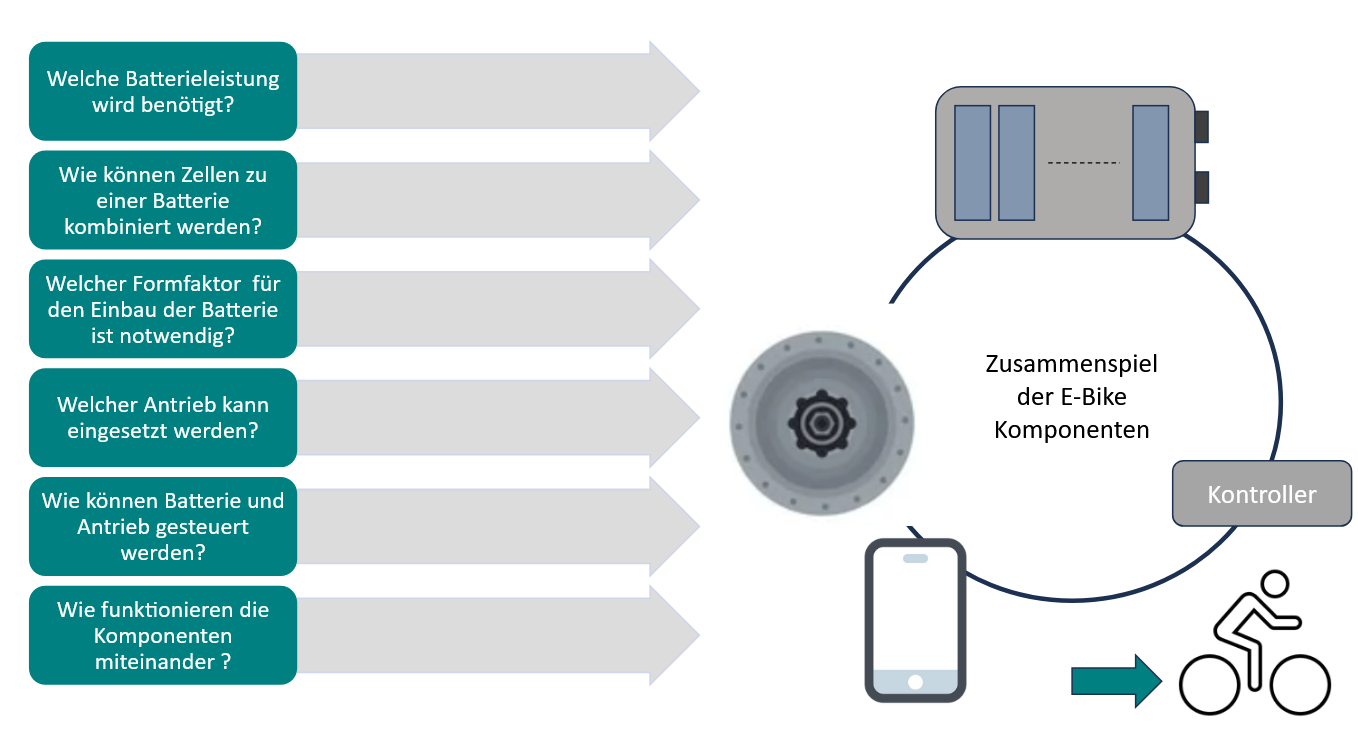
\includegraphics[width=11cm]{images/Flussdiagramm_E-bike.png}
    \caption{Zusammenspiel der E-Bike Komponenten}
    \label{fig:Komponenten}
\end{figure}


Diese wesentlichen Komponenten arbeiten zusammen, um ein E-Bike zu bilden, welches dem Fahrer elektrische Unterstützung beim Treten bietet und das Fahren erleichtert.
\chapter{Batterie bauen}
Eine der zentralen Komponenten bei der Konstruktion eines eigenen E-Bikes ist die Batterie, die den Motor mit Energie versorgt. In diesem Abschnitt werden wir uns eingehend mit der Herstellung einer maßgeschneiderten Lithium-Ionen-Batterie befassen, indem wir größere Zellen auswählen und in einer speziellen Konfiguration miteinander verbinden.\\

Für unsere Batterie greifen wir auf größere Lithium-Ionen-Zellen zurück, wobei die 21700-Zellen häufig bevorzugt werden. Diese speziellen Zellen verfügen über eine Nennspannung von 3,6 Volt. Ein E-Bike-Motor erfordert jedoch in der Regel eine höhere Spannung im Bereich von 36-42 Volt, um effizient zu funktionieren. Um diese Anforderung zu erfüllen, werden die 21700-Zellen in Serie geschaltet, wodurch ihre Einzelspannungen addiert werden.\\

Die Verbindung der Zellen erfolgt durch Löten, um eine solide und zuverlässige elektrische Verbindung sicherzustellen. Zusätzlich dazu wird ein Smart Battery Management System (BMS) eingesetzt, um die Batterie zu überwachen und zu schützen. Das BMS gewährleistet nicht nur die Sicherheit des Systems, sondern spielt auch eine entscheidende Rolle bei der effizienten Nutzung und Lebensdauer der Batterie. Es überwacht den Ladezustand der Zellen, verhindert Überladung und Tiefentladung sowie Temperaturabweichungen.\\

Die Konstruktion der Batterie ist ein entscheidender Schritt beim Bau eines selbstgemachten E-Bikes, da sie die Leistung und Reichweite des Fahrzeugs maßgeblich beeinflusst. In den folgenden Abschnitten werden wir uns weiteren Aspekten des E-Bike-Baus widmen, einschließlich der Programmierung des Controllers, der Anpassung der Gangschaltung und der Sicherstellung, dass das Fahrrad den erhöhten Anforderungen der elektrischen Unterstützung gerecht wird.\\ 
\section{Die Zellen}

%Größere Litiumionzellen bestellen aus einer vielzahl an Zellen hier werden meisten die 21700 Zellen verwendet.
%Diese haben eine Nennspannung von 3,6 Volt ein E-bike motor braucht meistens eine Spannung von 36-42V weswegen diese in Reihe geschaltet werden müssen.
%Die werden durch verlötung verbunden. Um Sicherung zu gewäreleisten wird ein \texttt{Smart Battery Managment System} verwendet. Dieses System verwaltet auch die Batterie.

\begin{itemize}
    \item Für welche Zellen sollte sich entschieden werden?
    \item Warum sollte eine von diesen Zellen gewählt werden?
    \item Was sind die Unterschiede zwischen den beiden Zellen?
\end{itemize}
% Für welche Zellen sollte gewähhlt werden?
%Warum sollte eine von diesen Zellen gewählt werden?
%Was sind die unterschiede zwischen den beiden Zellen?
Samsung 21700-40T Zelle \\
Samsung 21700-50E


\section{Anforderungen an die Batterie}
Fragen:
\begin{itemize}
    \item Was muss die Batterie leisten?
    \item Welche Parameter sind variabel?
    \item Welche Leistung sollte die Batterie haben?
    \item Welche Kapazität sollte die Batterie haben?
\end{itemize}

Parameter der Batterie
\begin{itemize}
    \item Volt/Spannung: 48V
    \item Ampher/Leistung: 20-36A wahrscheinlich nötig
    \item Ampherstunden/Kapazität: ca. 15-30Ah
\end{itemize}

Wie viele Zellen muss man in Reihe schalten damit die Spannung 48V beträgt:
\[ \frac{48V}{3.6V}\approx 13\]

Wie viele Zellen müssen Parallel geschaltet werden um auf die Leistung u. und Kapazität zu kommen:


13 in Reihe schalten
5 Parallel
65 Zellen

\section{Übersicht}
Ich habe noch ein paar Fragen zur Batterie, der Motor braucht wahrscheinlich 48V. Die Batterie wird wahrscheinlich aus den Samsung 21700-40T oder
Samsung 21700-50E Zellen gebaut werden. Für mein Rechenbeispiel werde ich die Samsung 21700-40T verwenden, diese hat die Parameter Spannung 3.6V, Entladestrom 9.8, Kapazität - mAh 4.900,00. Um auf ca. 48V zu erreichen, müssen 13 in Reihe geschaltet werden. Und je nachdem, welchen Entladestrom oder Kapazität benötigt werden müssen mehrere Zellen pro Reihe parallel geschaltet werden. Ein normaler E-Bike/S-Pedelec Akku hat eine Kapazität von 10-30Ah Stunden. Der Motor hat voraussichtlich eine Leistung von 1500W, wenn drei Zellen parallel geschaltet sind gibt es einen entladestrom von 29,4 bei einer Spannung von 48V kommt man auf eine Leistung der Batterie von 1375,92W(29,4A*3,6V*13). Man hätte eine Kapazität von 14,7 Ah. \\
 
Must-have
\begin{itemize}
    \item Zellen /////
    \item BMS (z.B. 60A, 10S) 10S heißt 10 in Reihe in meinem Fall waere es 13S /////
    \item Ladegeraet
    \item Doppelseitiges Klebeband
    \item Lade und entlade anschluss
    \item Kaptontape /////
    \item Kummiabdeckungen für den Pluspol /////
    \item Kupferdraht /////
    \item 
\end{itemize}

Offene Fragen
\begin{itemize}
    \item Wie kann die Verbindung am besten zwischen den Zellen herstellt werden ?
    \item Könnten auch gebrauchte Zellen verwendet werden?
    \item Wie muss es genau verbunden werden?
    \item Wo gehen die Kabel hin die aus dem Akku heraus gehen? An welche Adapter wird welches Kabel angeschlossen?
    \item Wo bekomme ich ein Punktschweiß Geraete her?
\end{itemize}


Löten geht so wie in diesem Video mit Nickband
\url{https://www.youtube.com/watch?v=e67byImYuL0}

Oder so \url{https://www.youtube.com/watch?v=pptK4TTZr8Q}
Mit einem Draht

https://www.sunkko.net/blog/two-types-of-bmss-and-each-wiring-diagram/


\section{Ladegeraet}

\section{Wahl des BMS}

Ich habe die Lishen Zellen bestellt 65 davon ich will 5 von diesen Parallel schalten.
Für diese will ich folgendes BMS verwenden 
https://www.lithiumbatterypcb.com/product/13s-48v-li-ion-battery-pcb-board-54-6v-lithium-bms-with-60a-discharge-current-for-electric-motorcycle-and-e-scooter-protection-2-2-3-2-2-2-2-2/
Es ist ausgelegt auf eine Leistung von 60A 

13S5P 

Welches eine Leistung von 60 A ausgelegt ist 

\section{Adpter fuer die Batterie}
Welche Anschluesse hat die Batterie?


\section{Verbindung zwischen den Zellen}
Löten oder Punktschweißen

Löten nicht stabil zu hohe belastung auf den Zellen. Wiederstand an den Zellen ist sehr Hoch können auch durch brennen was aber nicht schlimm sein muss .
Wie Löten?
Es braucht einen recht hochen Querschnitt da die Zellen einen recht hochem Entladestrom leisten. Rechnung:
\begin{itemize}
    \item Meschisch nicht so stabil
    \item Wiederstang sehr hoch wenn nicht gut verlötet
    \item braucht mehr Platz
    \item braucht ewig
    \item man braucht einen hochen Querschnitt
\end{itemize}

Punktschweißen
\begin{itemize}
    \item standard
    \item geringe hitze aud den Batterien
    \item meschanisch stabiler
    \item geht schneller
    \item 
\end{itemize}
Dinge die man braucht:
\begin{itemize}
    \item 220v 3-6A puch buttom
    \item 10mm Kupferdraht
    \item 6mm Kupferdraht
    \item Wie funktioniert ein Trafo
\end{itemize}
\url{https://www.youtube.com/watch?v=o5eej4MSotk}
Wie funktioniert ein trafo
\url{https://www.youtube.com/watch?v=rTVu1lZMPG0}
Rechnung für den trafo

\section{Punktschweißgerät}
Wie funktioniert schweißen?
Welchen Strom braucht man dazu?
Wie funktioniert ein Trafo?
Wo bekommt man einen Trafo her ?
Wie entfernt man den Sekundären block?
Problem micht den Primären Block beschädigen
Wie winkelt man den den Sekundären Block?
Wie stellt man die Halterung her?
Welchen durchschnitt brauchen die Spitzen?
Welche Optionen gibt es anzuschalten?
...

\section{Schlatplan}
Batterien verbindungen mit Doppelseitigem Klebeband
 
Punktscheißen mit dünneren schienen da sonst kurz schluss
Punktscheiß gerät wird sehr Heiß 
spitzen verrutschen 
Taster bleibt an 
Holz gibt nach

Reihenschaltung ebensfalls 
Am gesammten Pulspol abgesichert 
dann das BMS angeschlossen die Temperatursensoren auf der Batterie verteilt
die veschieden drähte nachschalt plan auf der Batterie verteilen und durch messen 
ne Problemen selbst erneut verleuten

Dann anschließen und mit der App verbinden
Man musste noch schauen wo die alle drähter genau hin müssen

B- zu batterie Minus
C- zu Minus des verbrauchers
Puls der Batterie zum Puls des verbrauchers

Dannach mit kartonsche verwickelt
\section{Batterie Hülle}
https://www.youtube.com/watch?v=1WqAEA9_mMw
mehrer Optionen fertige hülle kaufen mit Nickel schreifen 
Oder selbst eine Box bauen aus holz oder 
eine Hülle aus dem 3d drucker



https://www.lithiumbatterypcb.com/product/13s-48v-li-ion-battery-pcb-board-54-6v-lithium-bms-with-60a-discharge-current-for-electric-motorcycle-and-e-scooter-protection-2-2-3-2-2-2-2-2/


https://www.lithiumbatterypcb.com/smart-bms-software-download/




\chapter{Controller programmieren}
Ein entscheidender Schritt bei der Herstellung eines maßgeschneiderten E-Bikes besteht darin, den Controller des Motors zu programmieren, um die Leistungsparameter anzupassen und die Fahrerfahrung zu optimieren. Diese Anpassungen können sowohl die Geschwindigkeit als auch die Effizienz des E-Bikes beeinflussen.\\

Es bietet sich die Möglichkeit, Open-Source-Software zu verwenden oder neue Features hinzuzufügen, um den Controller nach den eigenen Wünschen zu gestalten. Hier sind einige Ressourcen, die Ihnen bei der Programmierung Ihres Controllers behilflich sein können:\\

    1. Open-Source-Firmware für SxxS-Ktxx-Controller: Eine Möglichkeit, den Controller zu programmieren, besteht darin, auf Open-Source-Firmware zurückzugreifen. Diese Firmware bietet die Flexibilität, die Funktionen des Controllers anzupassen und neue Parameter einzustellen. Das Pedelecforum bietet eine umfassende Ressource zur Verfügung, die Sie bei der Anpassung Ihrer Controller-Firmware unterstützt. Hier finden Sie weitere Informationen.\\

    2. GitHub Repository für BMSBattery S-Controller Firmware: Eine weitere wertvolle Quelle ist das GitHub-Repository für die Firmware der BMSBattery S-Controller. Dieses Repository bietet eine Community-gesteuerte Plattform, auf der Sie auf bereits entwickelte Software zurückgreifen oder eigene Anpassungen vornehmen können.\\

Die Programmierung des Controllers eröffnet Ihnen die Möglichkeit, die Leistungsparameter Ihres E-Bike-Motors individuell anzupassen, sei es für eine höhere Geschwindigkeit, eine längere Reichweite oder eine bessere Steuerung. Es ist jedoch wichtig, dies mit Vorsicht zu tun, um die Sicherheit und Stabilität des E-Bikes nicht zu gefährden.\\


%Es ist möglich den Controller zu programmieren der die Funktiontionen man kann eine Open Sources Software dafür verwenden oder die neue feateurs dafür hinzufügen.
%\url{https://www.pedelecforum.de/wiki/doku.php?id=elektrotechnik:open_source_firmware_fuer_sxxs_ktxx_-controller}
%\url{https://github.com/stancecoke/BMSBattery_S_controllers_firmware/wiki}
\include{input/steuergerät}
\chapter{Motor}


Kapitel 5 widmet sich dem Motor, einem zentralen Bauteil im E-Bike-System.
Bei der Auswahl und Integration eines Motors sind mehrere wichtige Fragen zu berücksichtigen, um eine optimale Leistung und Kompatibilität sicherzustellen.
Im Folgenden werden diese Fragen detailliert behandelt, wobei besonderes Augenmerk auf die Auswahl des Motors, seine Abmessungen, die Passform am Fahrrad, die Leistung in Watt und die ideale Positionierung des Motors gelegt wird.
\section{Arten von Fahrradmotoren}
%Welche Arten von Motoren gibt es?
E-Bikes verwenden drei Hauptarten von Motoren.
Der Mittelmotor befindet sich im Bereich des Tretlagers und bietet eine ausgeglichene Gewichtsverteilung, ein natürlicheres Fahrgefühl und eine effiziente Kraftübertragung durch die Mitte des Rahmens.
Im Gegensatz dazu ist der Hecknabenmotor im Hinterrad integriert und ermöglicht eine einfache Installation, kann jedoch das zusätzliche Gewicht die Fahrstabilität beeinträchtigen.
Der Frontnabenmotor befindet sich im Vorderrad und bietet ebenfalls eine einfache Installation, aber ein erhöhtes Lenkerdrehmoment kann das Lenkverhalten beeinflussen.
Die Wahl des Motors hängt von den individuellen Vorlieben des Fahrers und den Fahranforderungen ab.
\begin{figure}[h]
    \centering
    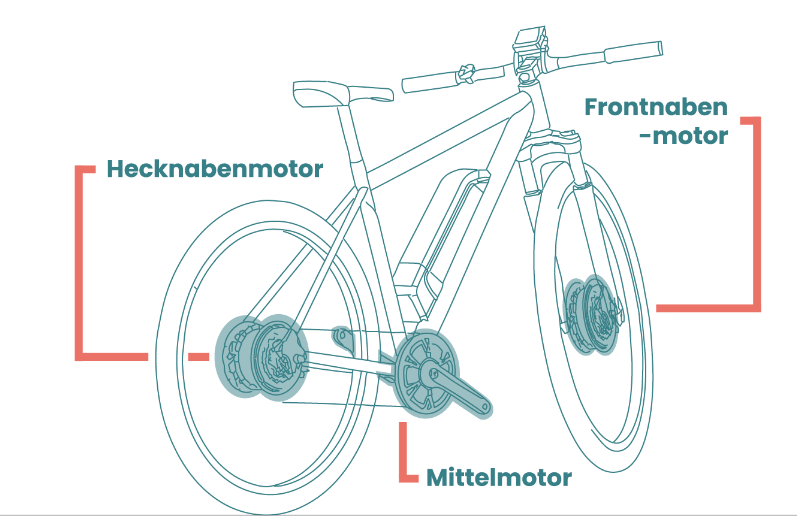
\includegraphics[width=10cm]{images/Motor_Arten}
    \caption{Motorenarten\cite{noauthor_e-bike_nodate}}%
    \label{fig:7}
\end{figure}
%Mittelmotor

\subsubsection*{Mittelmotor}
Ein Mittelmotor bei einem E-Bike befindet sich im Bereich des Tretlagers, also dort, wo üblicherweise auch die Kurbelgarnitur sitzt.
Im Gegensatz zu einem Heckmotor, der sich im Hinterrad befindet, oder einem Frontmotor, der sich im Vorderrad befindet, bietet ein Mittelmotor einige Vorteile:\\

Der Mittelmotor zeichnet sich durch eine ausgeglichenere Gewichtsverteilung aus, da er sich im Bereich des Tretlagers befindet.
Dadurch befindet sich der Schwerpunkt des Fahrrads näher am Boden, was zu einer besseren Fahrstabilität führt.
Dieses Merkmal ist besonders vorteilhaft beim Fahren auf unebenem Gelände oder in Kurven.
Zudem bietet der Mittelmotor ein natürlicheres Fahrgefühl, da er das Treten ähnlich wie ein herkömmliches Fahrrad unterstützt.\\

Ein weiterer Vorteil des Mittelmotors liegt in seiner Effizienz.
Durch die direkte Übertragung der Kraft auf das Antriebsritzel kann der Motor den Gangwechsel des Fahrers besser nutzen.
Dadurch wird die verfügbare Energie effizienter genutzt, was zu einer längeren Reichweite pro Akkuladung führen kann.
Schließlich trägt die zentrale Position des Motors im Rahmen zu einer besseren Gewichtsverteilung bei.
Im Vergleich zu einem Heckmotor, der das Gewicht eher auf der hinteren Seite des Fahrrads platziert, hilft der Mittelmotor dabei, das Fahrrad weniger unausgewogen zu machen und eine angenehmere Fahrt zu ermöglichen.\\

Ein Nachteil des Mittelmotors ist, dass der Verschleiß an den Ritzeln und der Kassette höher sein kann als bei anderen Antriebssystemen.
Dies liegt daran, dass der Motor direkt auf das Antriebsritzel wirkt und somit eine erhöhte Belastung auf die Zahnräder ausübt.
Insbesondere bei intensiver Nutzung und häufigen Schaltvorgängen kann dies zu einem schnelleren Verschleiß führen.
Es ist daher ratsam, regelmäßige Wartung durchzuführen und verschlissene Teile rechtzeitig auszutauschen, um die Lebensdauer des Antriebssystems zu maximieren und eine optimale Leistung zu gewährleisten.\\

Die Funktionsweise des Mittelmotors besteht darin, dass er die durch das Treten erzeugte Kraft des Fahrers verstärkt, indem er sie durch das Antriebsritzel auf das Hinterrad überträgt.
Dies geschieht normalerweise über ein System aus Zahnrädern und einer Kette oder einem Riemen.
Der Motor wird von der Energie aus einem Akku gespeist, der am Fahrrad angebracht ist und über eine Steuerungselektronik mit dem Motor verbunden ist.
Diese Elektronik regelt unter anderem die Leistung des Motors und kann oft auch verschiedene Fahrmodi und Assistenzniveaus bieten.

%Bild von mittelmotor
\begin{figure}[h]
    \centering
    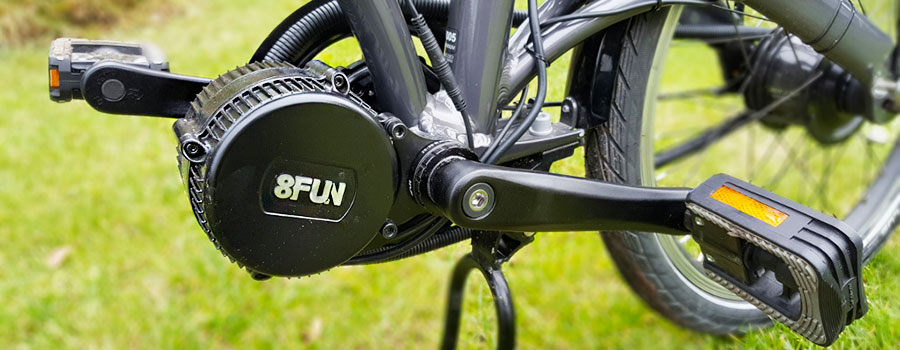
\includegraphics[width=10cm]{images/Mittelmotor-Fahrrad-nachruesten_F01.jpg}
    \caption{Mittelmotor\cite{noauthor_mittelmotor_nodate}}%
    \label{fig:8}
\end{figure}

\subsubsection*{Radnarbenmotor}
Der Nabenmotor ist in der Nabe des Hinterrads integriert und treibt dieses direkt an, wodurch die Kraftübertragung ohne Verluste direkt vom Motor auf das Laufrad erfolgt.
Ein Drehmomentsensor misst die Tretleistung des Fahrers und steuert die Motorunterstützung entsprechend.\\

Die Vorteile des Nabenmotors liegen im leisen Betrieb mit geringer Geräuschentwicklung, der Möglichkeit der Rekuperation zur Reichweitenerhöhung, der unauffälligen Integration in die Fahrradoptik und dem einfachen Einbau ohne spezielle Rahmenauslegung.\\

Jedoch weist der Nabenmotor auch einige Nachteile auf, wie eine ungünstige Gewichtsverteilung mit dem Schwerpunkt am Hinterrad, die Inkompatibilität mit Nabenschaltungen (nur Kettenschaltung möglich), die Tendenz zum Durchdrehen des Vorderrads bei Steigungen und Nässe, einen höheren Tretwiderstand durch das Getriebe im Hinterrad, problematischen Reifenwechsel durch integrierte Verkabelung und die Möglichkeit älterer Systeme, bei Dauerbelastung zu überhitzen.\\

Zusammengefasst bietet der Nabenmotor einen leisen Betrieb und Rekuperation, hat aber Nachteile bei der Gewichtsverteilung, Schaltübungskompatibilität und Lenkung, vor allem bei anspruchsvollem Gelände.\\

%Bild von Nabenmotor
\begin{figure}[h]
    \centering
    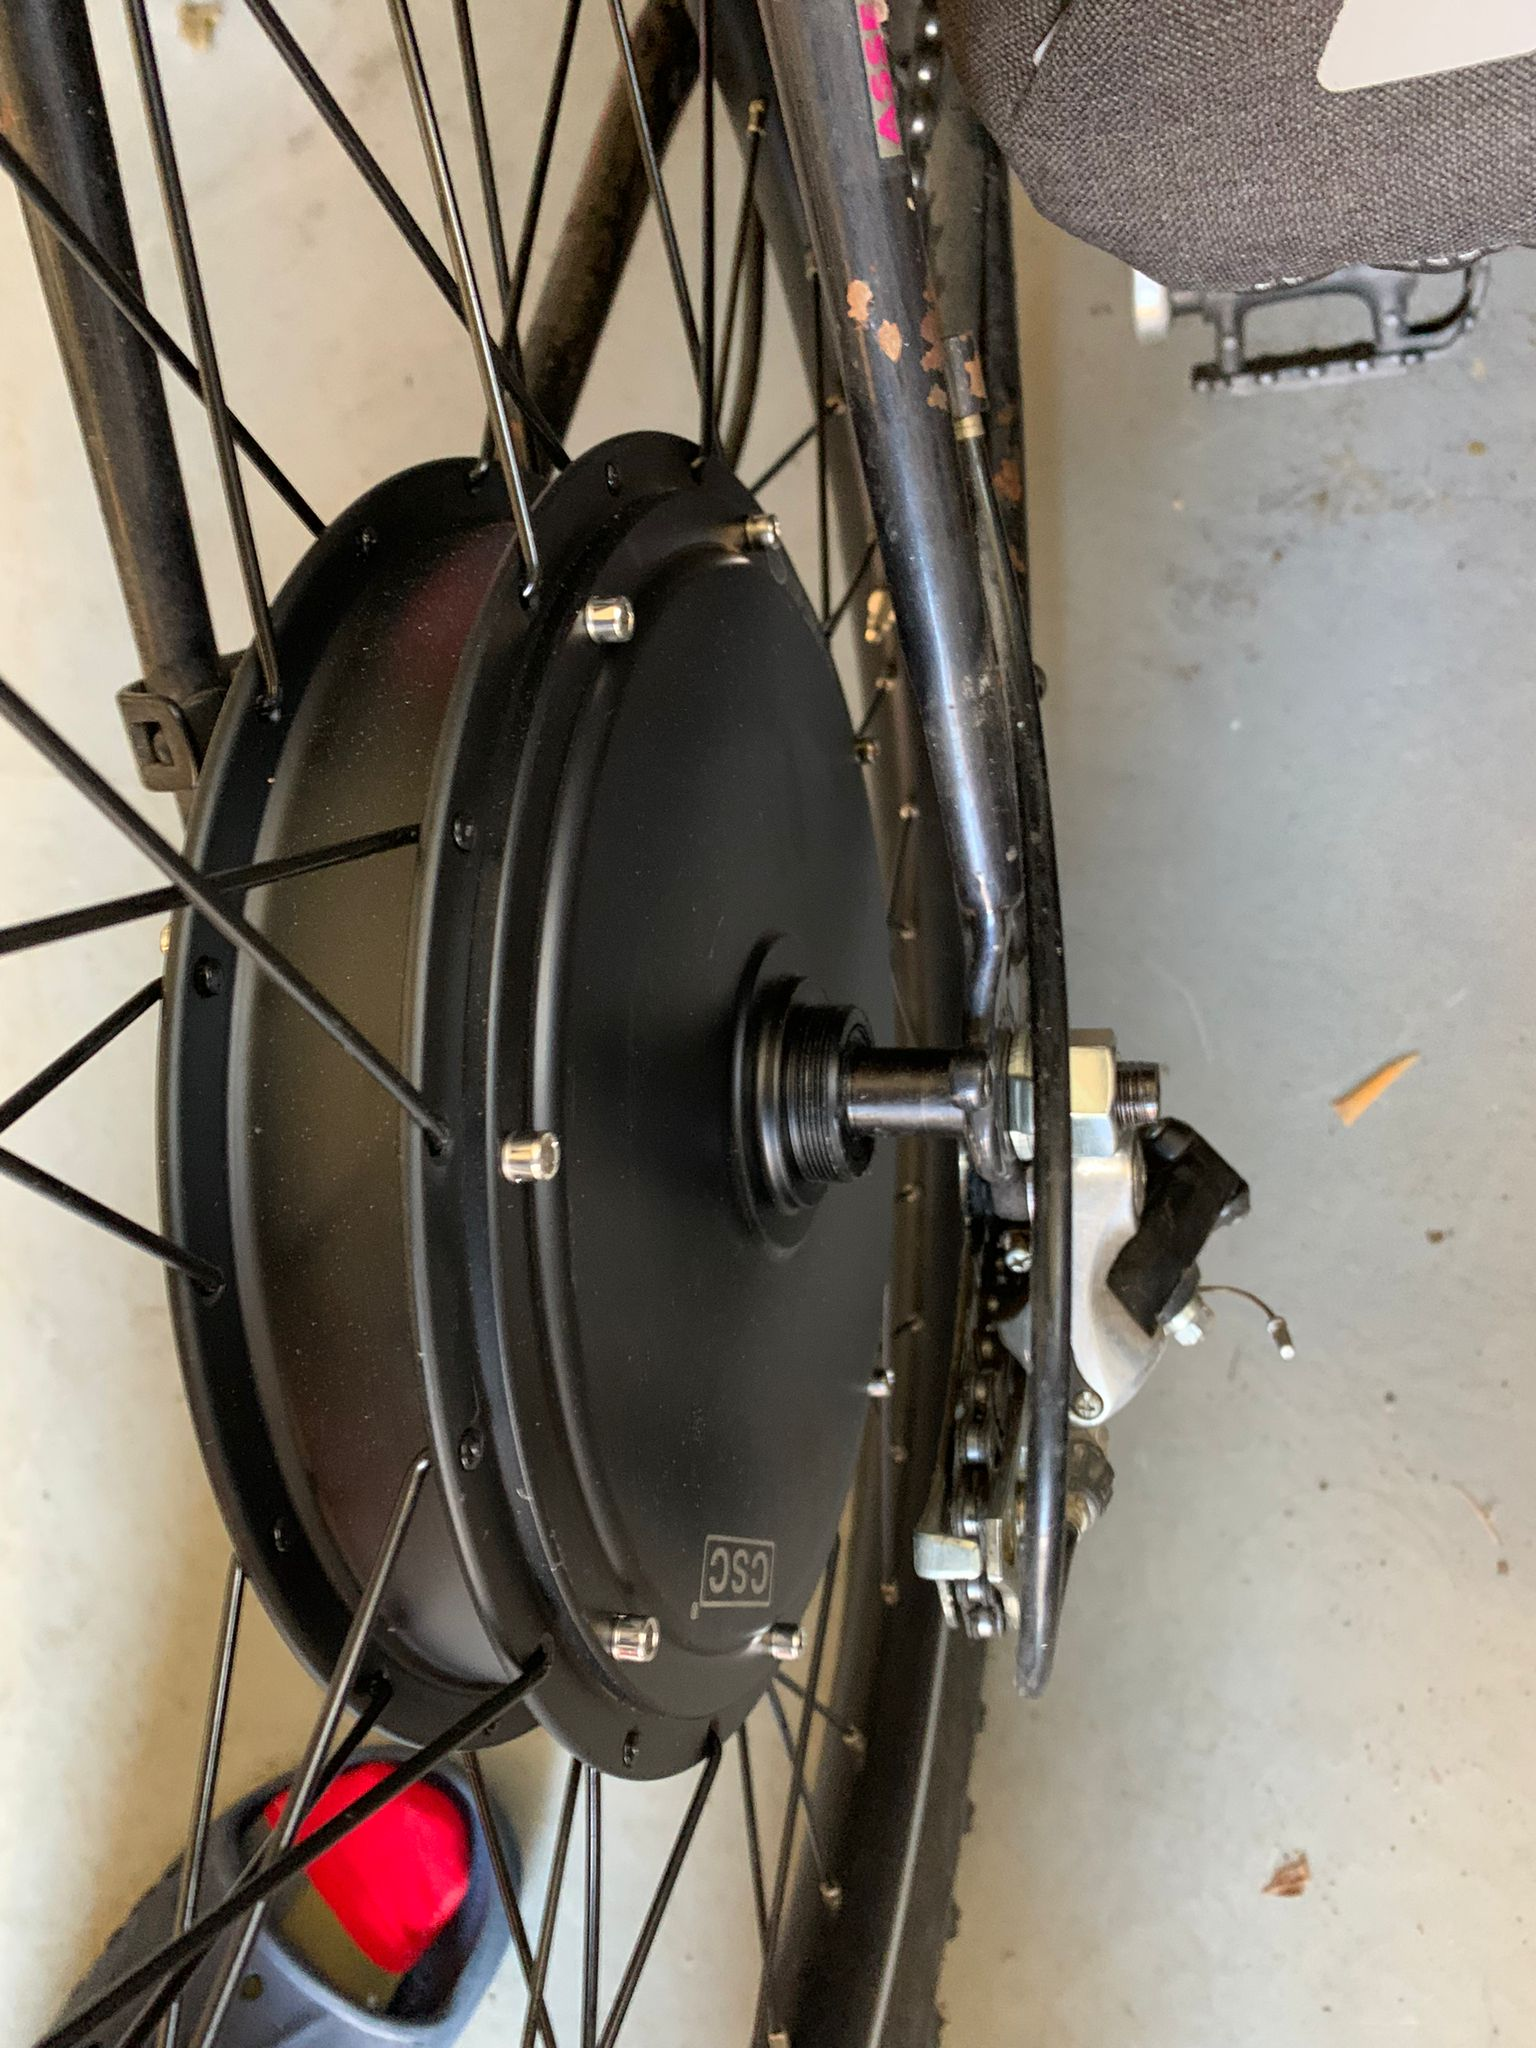
\includegraphics[width=10cm]{images/Radnabenmotor.jpg}
    \caption{Radnarbenmotor\cite{lorenz_scherrer_selbst_2023}}%
    \label{fig:9}
\end{figure}


Die Entscheidung für einen Nabenmotor basiert auf mehreren überzeugenden Argumenten.
Zunächst einmal ist die Installation eines Nabenmotors im Vergleich zu anderen Antriebssystemen, wie beispielsweise einem Mittelmotor, deutlich einfacher.
Da der Motor direkt in der Nabe des Rades integriert ist, erfordert seine Installation keine speziellen Rahmenanpassungen oder komplexe Montageprozesse.
Dies macht den Einbau sowohl für Hersteller als auch für Endbenutzer unkompliziert und kostengünstig.\\

Ein weiterer Vorteil des Nabenmotors liegt in seiner dezenteren Integration in das Design des Fahrrads.
Da der Motor im Inneren der Nabe verborgen ist, ist er für Außenstehende weniger sichtbar und beeinträchtigt nicht das ästhetische Erscheinungsbild des Fahrrads.
Diese unauffällige Integration kann besonders für Fahrer wichtig sein, die ein elegantes und minimalistisches Design bevorzugen.\\

Darüber hinaus weist der Nabenmotor tendenziell einen geringeren Verschleiß auf als andere Antriebssysteme.
Da die Kraftübertragung direkt vom Motor auf das Laufrad erfolgt, gibt es weniger bewegliche Teile und somit weniger Anfälligkeit für Verschleißerscheinungen.
Dies führt zu einer längeren Lebensdauer des Antriebssystems und reduzierten Wartungskosten für den Fahrer.\\

Schließlich bietet der Nabenmotor ein großes Potenzial für Leistung.
Durch die direkte Kraftübertragung auf das Laufrad und die Möglichkeit einem hohen Drehmoment entwicklung kann der Nabenmotor beeindruckende Leistungen erbringen, insbesondere im Hinblick auf Beschleunigung und Bewältigung von Steigungen.
Diese Leistungsstärke macht den Nabenmotor zu einer attraktiven Option für Fahrer, die hohe Leistung und Effizienz von ihrem E-Bike erwarten.\\

Insgesamt bietet der Nabenmotor eine Reihe von überzeugenden Vorteilen, darunter eine einfache Installation, dezente Integration, geringeren Verschleiß und beeindruckende Leistungsfähigkeit.
Diese Argumente machen ihn zu einer attraktiven Wahl für diejenigen, die nach einem zuverlässigen und leistungsstarken Antriebssystem für ihr E-Bike suchen.\\
\subsubsection*{Funktionsweise eines Bürstenlosen Gleichstrommotors}


Bei den Radnarbenmotoren handelt es sich um einen Bürstenlosen Gleichstrommotor.
Der Motor wandeln elektrische Energie in mechanische um.

%Konstruktion von einem Bürstenlosen
%Der Motor besteht aus einenm rotor stator
Bürstenlose Gleichstrommotoren (BLDC-Motoren) gehören zu den effizientesten und leistungsstärksten Antriebslösungen in der heutigen Industrie.
Sie bestehen aus einem Rotor und einem Stator, wobei der Stator die feststehende Komponente und der Rotor die sich drehende ist.
Links ist der Rotor zusehen und recht der Stator \ref{fig:11}

\begin{figure}[h]
    \centering
    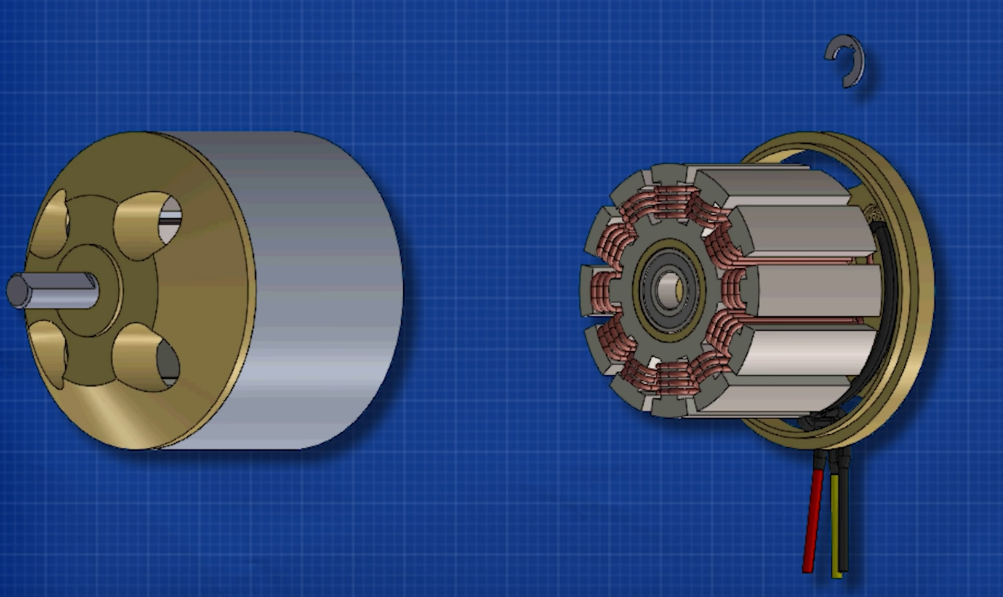
\includegraphics[width=10cm]{images/RotorStator.png}
    \caption{Rotor und Stator\cite{ingenieursmentalitat_burstenloser_2022}}%
    \label{fig:11}
\end{figure}

%Was bedeuteten Zähne des Stators?
Die Zähne des Stators sind die hervorstehenden Teile des Statorblechs, die dazu dienen, die Spulen zu umgeben und zu führen.
Sie sind strategisch angeordnet, um ein magnetisches Feld zu erzeugen, das den Rotor antreibt.  \ref{fig:11}\\

%Was machen die Spulen? und in welche Phasen gruppen sind sie aufgeteilt?
Die Spulen im Stator sind für die Erzeugung des magnetischen Feldes verantwortlich, das den Rotor antreibt.
Sie sind in drei Phasengruppen unterteilt: U, V und W. Diese Phasengruppen sind jeweils um 120 Grad versetzt, um ein gleichmäßiges Drehmoment zu erzeugen.\\

%Warum sind die benachbarten Spulen in verschiedene Richtungen gewickelt?
%Was bedeutet dlrk-Wicklung?
Die benachbarten Spulen sind in verschiedene Richtungen gewickelt, um sicherzustellen, dass sich das magnetische Feld gleichmäßig um den Rotor verteilt und somit ein reibungsloser Betrieb gewährleistet ist.
Diese Wickeltechnik wird auch als dlrk-Wicklung bezeichnet \ref{fig:12}.\\

\begin{figure}[h]
    \centering
    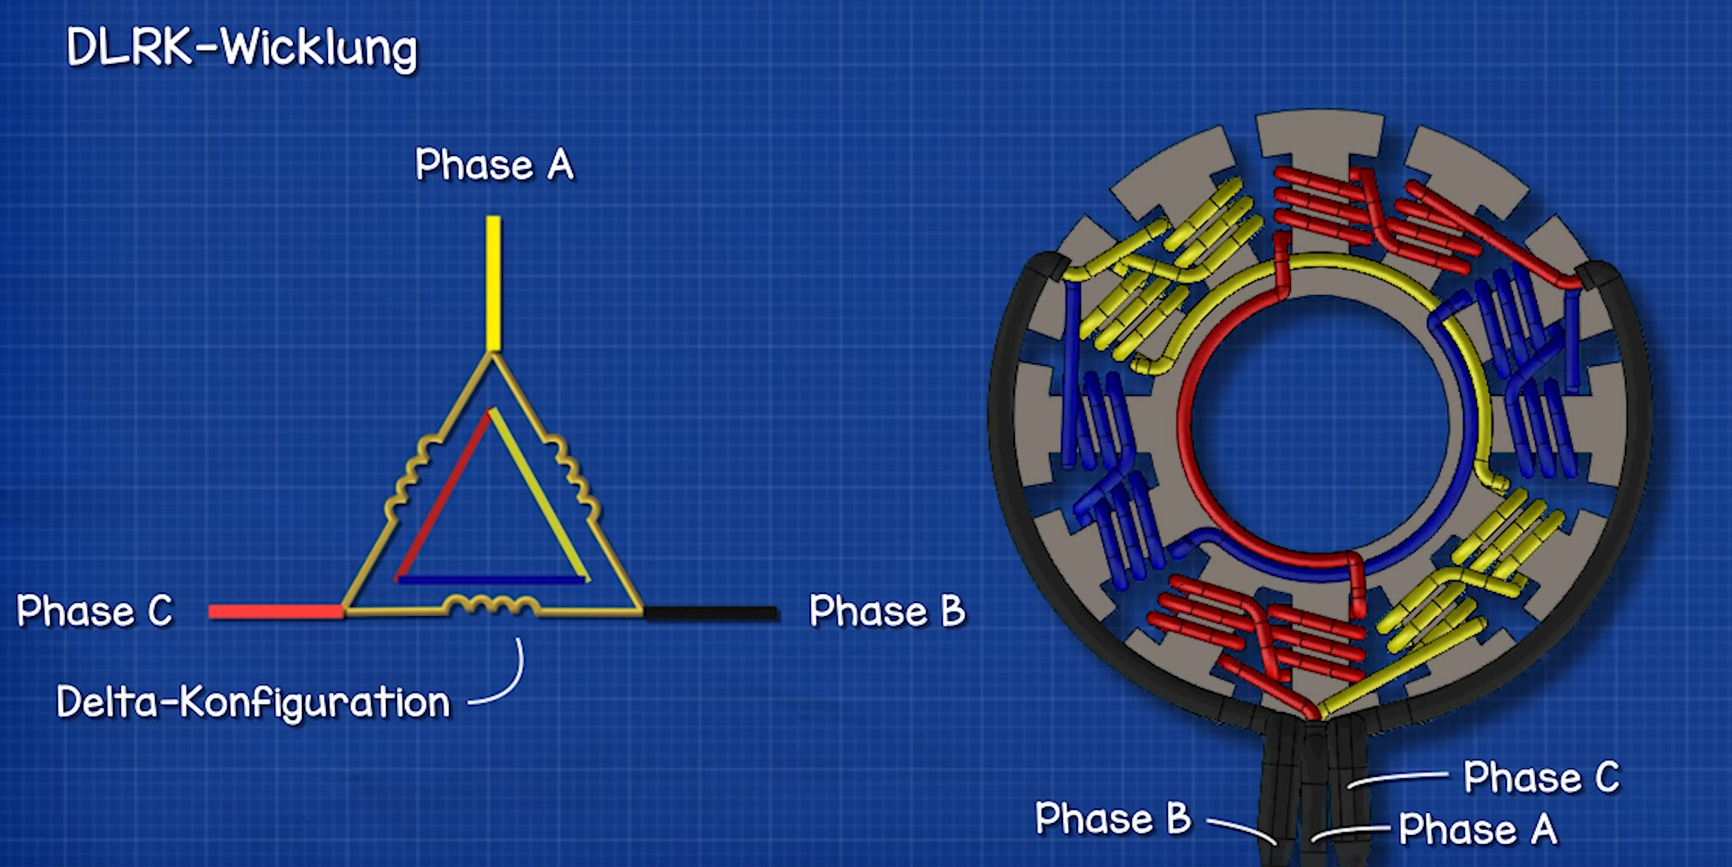
\includegraphics[width=10cm]{images/DLRK-Wicklung.png}
    \caption{DLRK-Wicklung\cite{ingenieursmentalitat_burstenloser_2022}}%
    \label{fig:12}
\end{figure}

%wue sind die permatnet magneten am Rotor angebracht?
Die Permanentmagnete am Rotor sind so angebracht, dass sie eine feste und starke magnetische Kraft erzeugen.
Sie sind in einer bestimmten Anordnung platziert, um ein optimales magnetisches Feld zu erzeugen und somit eine effiziente Drehbewegung zu ermöglichen.\\
%Wie sind sie anbracht?
%Die anzahl der Magneten und spulen unterscheiden sich damit sie sich nicht ausrichten
Die Anzahl der Magneten und Spulen kann variieren, um sicherzustellen, dass sich diese nicht ausrichten und somit das gewünschte Drehmoment erzeugt wird.
Durch diese Unterschiede in der Anordnung wird eine gleichmäßige und stabile Leistung des Motors gewährleistet.\\

%Funktionsweise


%Bild von Nabenmotor


%ein BLDC_Motor vs ein DC-Motor


\subsection{Energierückgewinnung}

Radnabenmotoren bieten einen weiteren Vorteil: die Stromrückgewinnung.
Durch ihre Konstruktion ermöglichen sie es, kinetische Energie während des Bremsens in elektrische Energie umzuwandeln.
Dies geschieht, indem der Motor als Generator fungiert.

Der BLDC-Motor, der in Radnabenmotoren verwendet wird, kann seine Rolle ändern und als Generator arbeiten, wenn er dem Drehmoment entgegenwirkt.
Bei dieser Umkehrung des Betriebsmodus des Motors wird die mechanische Energie des rotierenden Rades in elektrische Energie umgewandelt, die dann in einer Batterie gespeichert oder direkt verwendet werden kann.
Diese Stromrückgewinnungsfunktion ist besonders nützlich in Anwendungen, in denen häufiges Bremsen oder Abbremsen erforderlich ist, wie zum Beispiel bei Elektrofahrrädern.
Sie trägt nicht nur zur Verbesserung der Energieeffizienz bei, sondern kann auch die Reichweite des Fahrzeugs erhöhen und die Lebensdauer der Bremsen verlängern, da weniger mechanische Bremsen verwendet werden müssen.
Zudem vergessert sie den Bremsweg des E-Bikes.

%\href{https://www.portescap.com/de-DE/wissen/dokumente-und-zeichnungen/white-papers/nutzung-eines-gleichstromb%C3%BCrstenmotors-als-generator}

%Im Controller ist wahrscheinlich ein gleich Spannungsrichter der die Spannung und die Stromstärke wieder an die Batterie weitergibt


\section{Position des Motors}
%Vorderrad oder Hinterradantrieb?
Die Wahl zwischen einem Vorderrad- oder Hinterradmotor bei einem E-Bike hängt von verschiedenen Faktoren ab, die sowohl die Leistung als auch das Fahrverhalten des Fahrrads beeinflussen können.
Beginnen wir mit dem Vorderradmotor: Ein klarer Vorteil liegt in der schnellen Umsetzbarkeit des Umbaus.
Die Installation gestaltet sich vergleichsweise einfach, da der Motor direkt in die Nabe des Vorderrads integriert wird.
Dies ermöglicht eine rasche Anpassung von herkömmlichen Fahrrädern zu E-Bikes.\\

Jedoch weist der Vorderradmotor einige Nachteile auf.
Aufgrund der direkten Kraftübertragung auf das Vorderrad kommt es schnell zum Durchdrehen, insbesondere auf rutschigem Untergrund oder bei Steigungen.
Dies beeinträchtigt das Fahrverhalten und die Traktion des Vorderrads negativ.
Darüber hinaus ist die Gewichtsverteilung problematisch, da ein Großteil des zusätzlichen Gewichts durch den Motor vorne am Fahrrad konzentriert ist.
Dies kann zu einem ungleichmäßigen Fahrgefühl führen, insbesondere bei höheren Geschwindigkeiten oder in Kurven.\\

Um diese potenziellen Probleme zu untersuchen, wurden zwei Experimente durchgeführt.
Diese Experimente zielen darauf ab, das Durchdrehen des Vorderrads unter verschiedenen Bedingungen zu untersuchen und die Auswirkungen auf das Fahrverhalten zu bewerten.
Die Ergebnisse dieser Experimente liefern wertvolle Erkenntnisse für die Entscheidungsfindung bei der Wahl des Motors.\\

Auf der anderen Seite steht der Hinterradmotor, der seine eigenen Vor- und Nachteile bietet.
Einer der offensichtlichen Nachteile ist die komplexere Installation im Vergleich zum Vorderradmotor.
Da der Motor in die Nabe des Hinterrads integriert wird, erfordert die Installation möglicherweise spezielle Anpassungen des Rahmens und der Verkabelung.
Dies kann zu einem längeren Installationsprozess führen und zusätzliche Kosten verursachen.\\

Darüber hinaus kann der Hinterradmotor die Kompatibilität mit Nabenschaltungen einschränken, da die meisten Hinterradmotoren nur mit Kettenschaltungen kompatibel sind.
Dies kann die Auswahl an verfügbaren Schaltung- und Gangoptionen für den Fahrer begrenzen.
Zudem kann der Einbau des Motors zu einem höheren Tretwiderstand führen, da das Getriebe im Hinterrad zusätzlichen Widerstand erzeugen kann.\\

Trotz dieser Nachteile bietet der Hinterradmotor auch einige wichtige Vorteile.
Die Gewichtsverteilung ist oft besser ausgeglichen als beim Vorderradmotor, da sich der Motor im hinteren Teil des Fahrrads befindet.
Dies kann zu einem stabileren Fahrverhalten beitragen, insbesondere bei höheren Geschwindigkeiten oder in Kurven.
Darüber hinaus ermöglicht die Integration des Motors in das Hinterrad eine unauffälligere Optik, da der Motor weniger sichtbar ist und das ästhetische Erscheinungsbild des Fahrrads weniger beeinträchtigt wird.\\

Die Entscheidung für einen Hinterradmotor wurde letztendlich aufgrund dieser verschiedenen Faktoren und den Ergebnissen der zwei Experimente getroffen.
Trotz der komplexeren Installation bietet der Hinterradmotor eine bessere Gewichtsverteilung, eine stabilere Fahrdynamik und eine unauffälligere Optik, was ihn zu einer attraktiven Option für viele Fahrradfahrer macht.\\
%Vorteile und nachteile

\section{Leistung des Motors}

Die Entscheidung über die Motorleistung für den Bau eines E-Bikes ist ein wichtiger Schritt, der sorgfältige Überlegungen erfordert.
Dabei müssen mehrere Faktoren berücksichtigt werden, um die optimale Leistung zu bestimmen.\\

Zunächst ist es wichtig zu erwähnen, dass das E-Bike nicht in seiner vorgefertigten Form gekauft werden kann, was bedeutet, dass der Motor separat erworben werden muss.
Dies eröffnet verschiedene Möglichkeiten für den Erwerb und die Installation des Motors.
Eine Möglichkeit besteht darin, einen Motor zu kaufen, an dem bereits Speichen und Felge angebracht sind, während eine andere Möglichkeit darin besteht, nur den Motor zu erwerben und Speichen sowie Felge selbst anzubringen.
Beide Optionen haben ihre Vor- und Nachteile.\\

Beim selbstständigen Anbringen von Speichen und Felge ist die Entscheidungsfreiheit hinsichtlich des Motors flexibler.
Allerdings geht dies mit zusätzlichem Arbeitsaufwand einher und birgt das Risiko, dass die Zusammenstellung möglicherweise nicht in der Lage ist, die auf den Motor ausgeübte Kraft zu bewältigen.
Im Gegensatz dazu kann bei einem vollständigen Motor mit Speichen und Felge davon ausgegangen werden, dass die Zusammenstellung die Kraftauswirkung aushält.\\

Nachdem diese Kriterien definiert wurden, wurde eine Marktanalyse durchgeführt, um festzustellen, welche Optionen verfügbar sind.
Basierend auf den identifizierten Anforderungen und den verfügbaren Optionen wurde die Entscheidung getroffen, einen 1500 Watt-Motor zu verwenden.
Diese Leistungseinstellung ermöglicht eine angemessene Motorleistung für das E-Bike, ohne dabei die Strukturintegrität des Fahrzeugs zu gefährden.
Durch die Verwendung eines Motors mit dieser Leistung kann eine ausreichende Unterstützung für das E-Bike gewährleistet werden, während gleichzeitig potenzielle Schäden vermieden werden.\\


%\section{Reichweite}
%Reichweite berechnen

%Es muss noch ein experiment gemacht werden





\include{input/Schaltung}
\chapter{Konstruktion}

Die Konstruktion des E-Bikes begann mit einer gründlichen Analyse der benötigten Komponenten und deren Positionierung, einschließlich der Batterie, des Motors und des Controllers.
Um die optimale Platzierung zu ermitteln, wurde zunächst ein Test mit einem verfügbaren Laufrad durchgeführt, welches sich als geeignete Testplattform erwies.

\section{Positionierung der Komponenten}

Für den Antrieb wurde zunächst ein Frontantrieb in Betracht gezogen und getestet, dies führte jedoch zu unerwünschtem Durchdrehen des Rades, selbst bei geringer Leistung von nur 50\%.
Daraufhin wurde die Batterie in der Mitte des Rahmens positioniert, um eine gleichmäßige Gewichtsverteilung zu gewährleisten,
dies erwies sich dynamischer, als auch aus statischer Sicht vorteilhafter.
Siehe Bild~\ref{fig:27}.
\begin{figure}[h!]
    \centering
    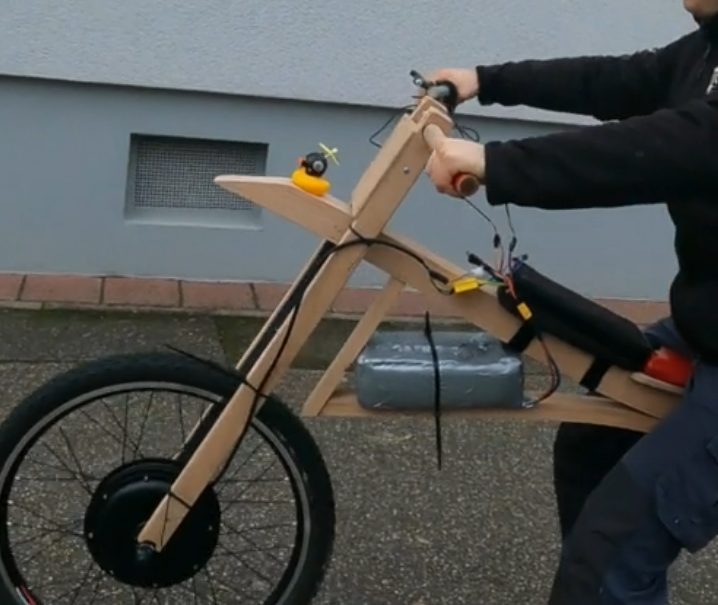
\includegraphics[width=8cm]{images/Bild des Laufrads}
    \caption{Laufrader Test\cite{lorenz_scherrer_selbst_2023}}
    \label{fig:27}
\end{figure}


Schließlich wurde die Entscheidung getroffen, den Motor am Hinterrad anzubringen, und die Batterie weit vorne am Rahmen zu platzieren, um das Gewicht auszubalancieren, insbesondere aufgrund des schweren Hinterradantriebs. 
Der Controller wurde an der hinteren Flaschenhalterung montiert, dies erweist als funktional.
Der Controller und das gesamte Fahrrad sind in Abbildung\ref{fig:28} zu sehen.


\begin{figure}[h!]
    \centering
    \includegraphics[width=8cm]{images/Bild des Fahrrads}
    \caption{Kompletes Fahrrad\cite{lorenz_scherrer_selbst_2023}}
    \label{fig:28}
\end{figure}


Für die Befestigung der Batterie wurde robustes Stahlblech verwendet, das sorgfältig gebogen und mit einer Schlaufe gesichert wurde.
Dieser Bügel wurde am vorderen Getränkehalter angebracht, um das Gewicht gleichmäßig zwischen dem Hinterrad-Antrieb zu verteilen.
Obwohl diese Befestigungsmethode sich als nicht ganz stabil erwies und die Batterie während des Tests herunterfiel, konnte sie dennoch vorübergehend gesichert werden.
Im nachfolgen Bild\ref{fig:29} ist die Montage dargestellt.
\begin{figure}[h!]
    \centering
    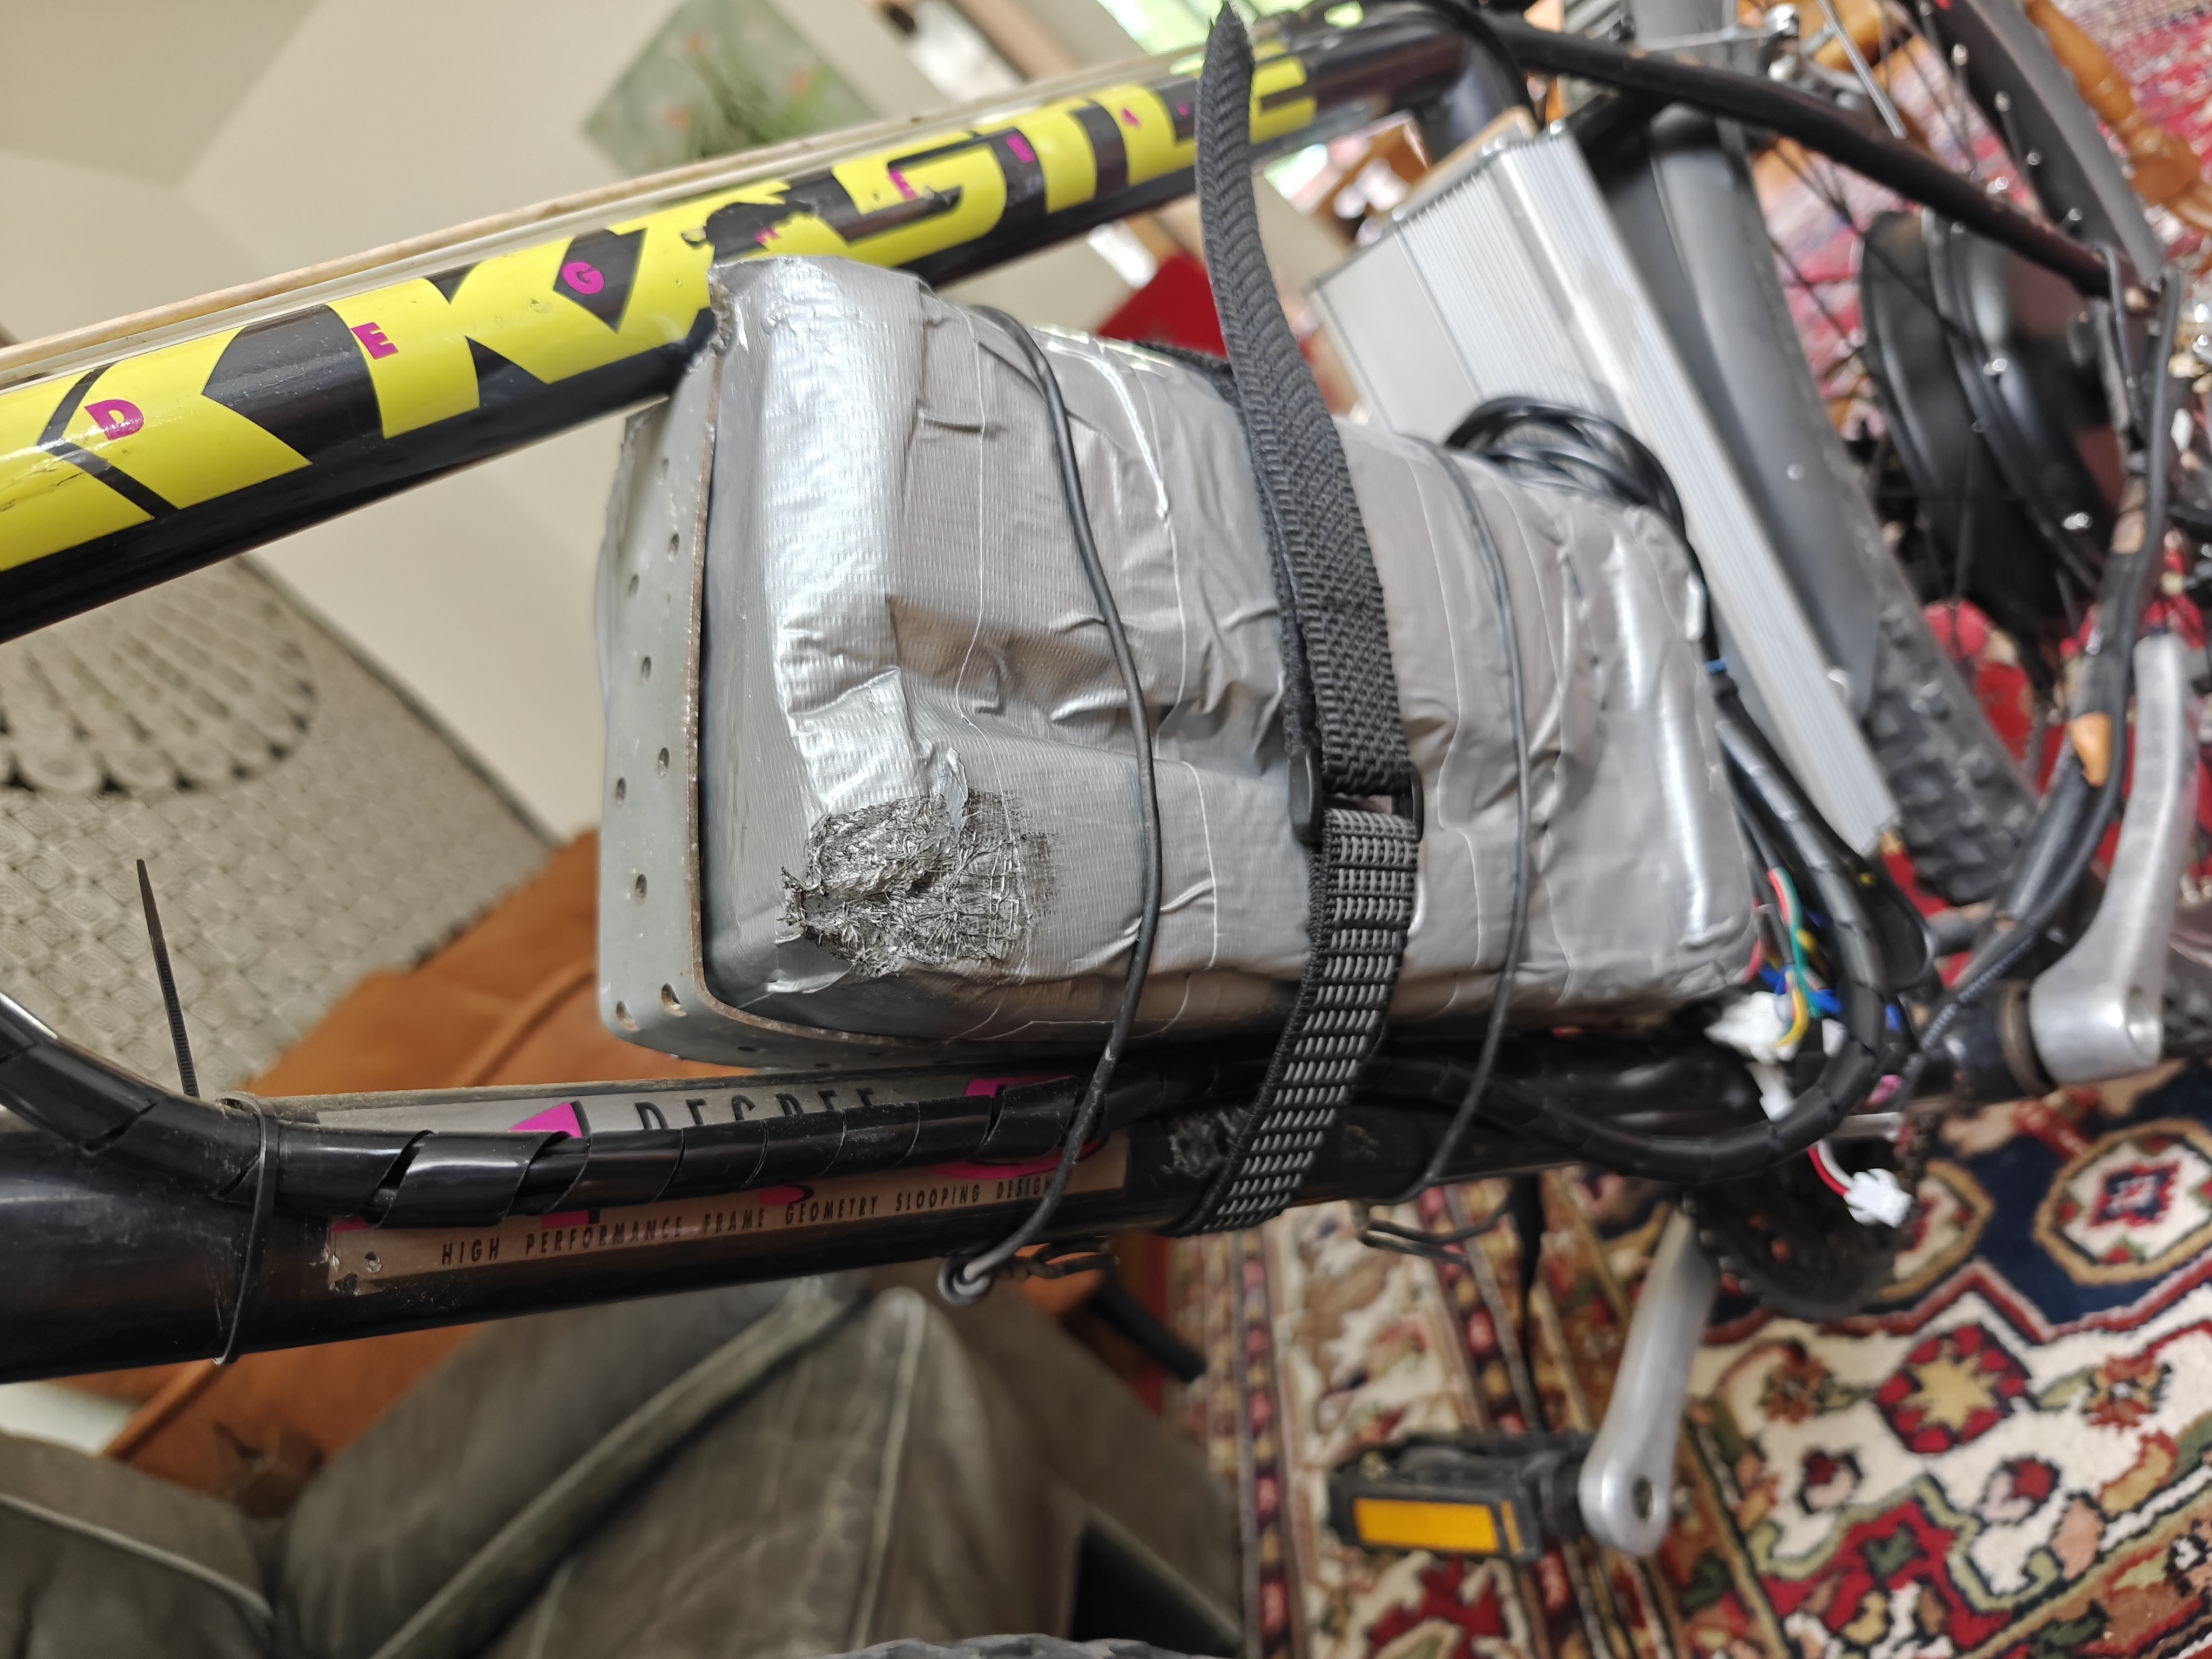
\includegraphics[width=8cm]{images/Bild der Batterie am Fahrrad}
    \caption{Batterie montiert\cite{lorenz_scherrer_selbst_2023}}
    \label{fig:29}
\end{figure}


Die Verkabelung erfolgte anschließend.
Wobei die Bremsen durch elektrische Bremsen ersetzt wurden, das Drehgas und das Display hinzugefügt wurden.
Die Kabelführung wurde mit einem Spiralkanal und Kabelbindern umgesetzt.
Es wurde darauf hingewiesen, dass der PSA-Sensor während des Projekts nicht hinzugefügt werden konnte~\ref{fig:28}.






\section{Montage des Motors}


Die Montage des Motors erfolgte im Anschluss an die Positionierung der Batterie und des Controllers. 
Ein wichtiger Schritt dabei war die korrekte Befestigung der Motorachse.
Es wurden zwei Muttern verwendet, die fest angezogen wurden. 
Allerdings stellte sich heraus, dass insbesondere bei leistungsstarken Motoren mit einer Leistung von 1500 Watt, die Belastung für die Achse zu hoch sein kann.
Das aufgebaute Drehmoment kann dazu führen, dass die Achse bricht. 
Aus diesem Grund wurde ein Torque Arm verwendet, um die Achse zu verstärken. 
Eine visuelle Darstellung dieses Vorgangs ist im Bild unten dargestellt~\ref{fig:30}.

\begin{figure}[h!]
    \centering
    \includegraphics[width=8cm]{images/Bild des Motors}
    \caption{Motor montiert\cite{lorenz_scherrer_selbst_2023}}
    \label{fig:30}
\end{figure}


Die Befestigungsschlaufe erwies sich als etwas zu dünn, weshalb zusätzliche Stäbe eingefügt wurden, um die Stabilität zu erhöhen.
Trotz dieser Anpassungen funktionierte die Montage des Motors insgesamt gut.
Die Bremsbacken mussten an die Felge angepasst werden, wobei festgestellt wurde, dass die Rekuperationsbremse deutlich stärker ist als die konventionelle Bremse.
Dies erwies sich als vorteilhaft, um die letzten Kilometer pro Stunde zu reduzieren, vornehmlich bei niedrigen Geschwindigkeiten, bei der Rekuperationsbremse nicht mehr so effektiv ist.
Dennoch erwiesen sich die Bremsbacken als effektiv und wurden sowohl vorne als auch hinten entsprechend angepasst.




% Ab hier beginnt der Anhang
\appendix
\addcontentsline{toc}{chapter}{Anhang}



\chapter*{Anhang}
\begin{landscape}
    % Hier kommt der Inhalt, den du drehen möchtest


\begin{figure}[h]
    \centering
    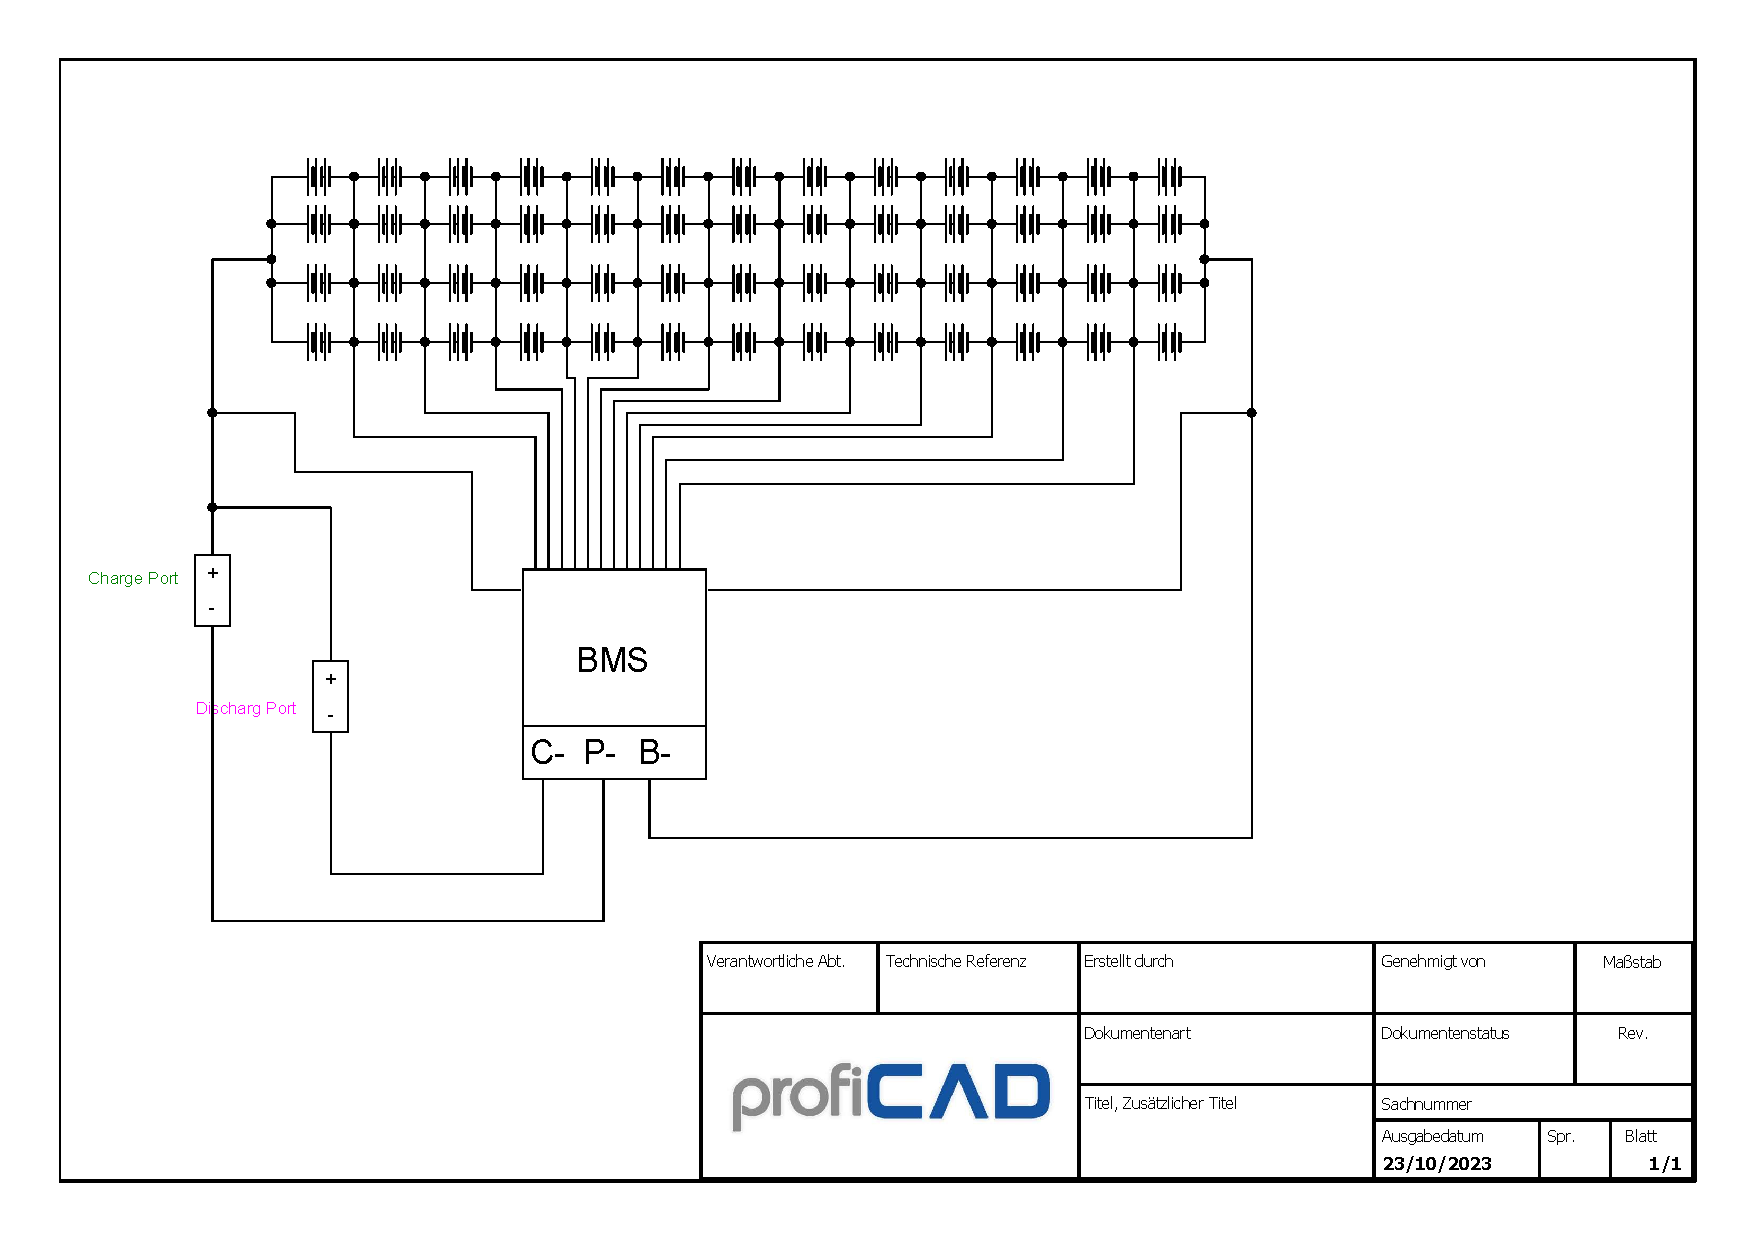
\includegraphics[width=22cm]{images/Schaltplan.pdf}
    \caption{Schaltplan\cite{lorenz_scherrer_selbst_2023}}%
    \label{fig:5_1}
\end{figure}
\end{landscape}

\begin{figure}[h]
    \centering
    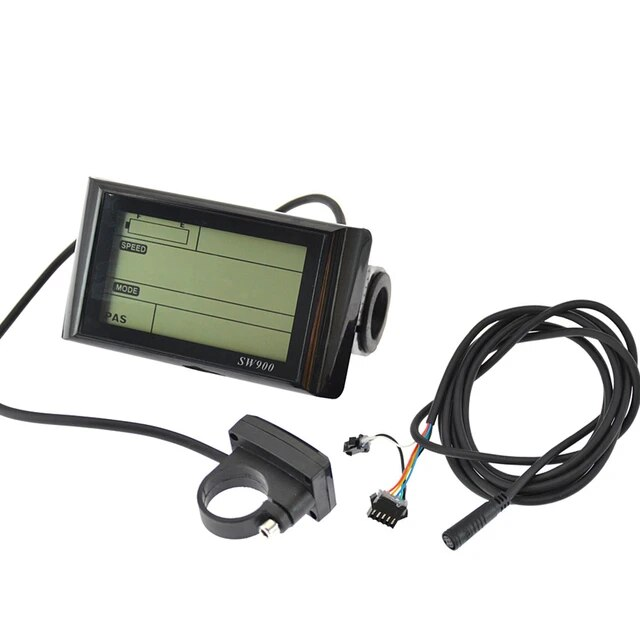
\includegraphics[width=10cm]{images/sw900.jpeg}
    \caption{sw900\cite{lorenz_scherrer_selbst_2023}}%
    \label{fig:15}
\end{figure}


\begin{figure}[h]
    \centering
    \includegraphics[width=10cm]{images/RasenmäherAkku}
    \caption{Rasenmäher Akku\cite{lorenz_scherrer_selbst_2023}}
    \label{fig:20}
\end{figure}

\begin{figure}[h]
    \centering
    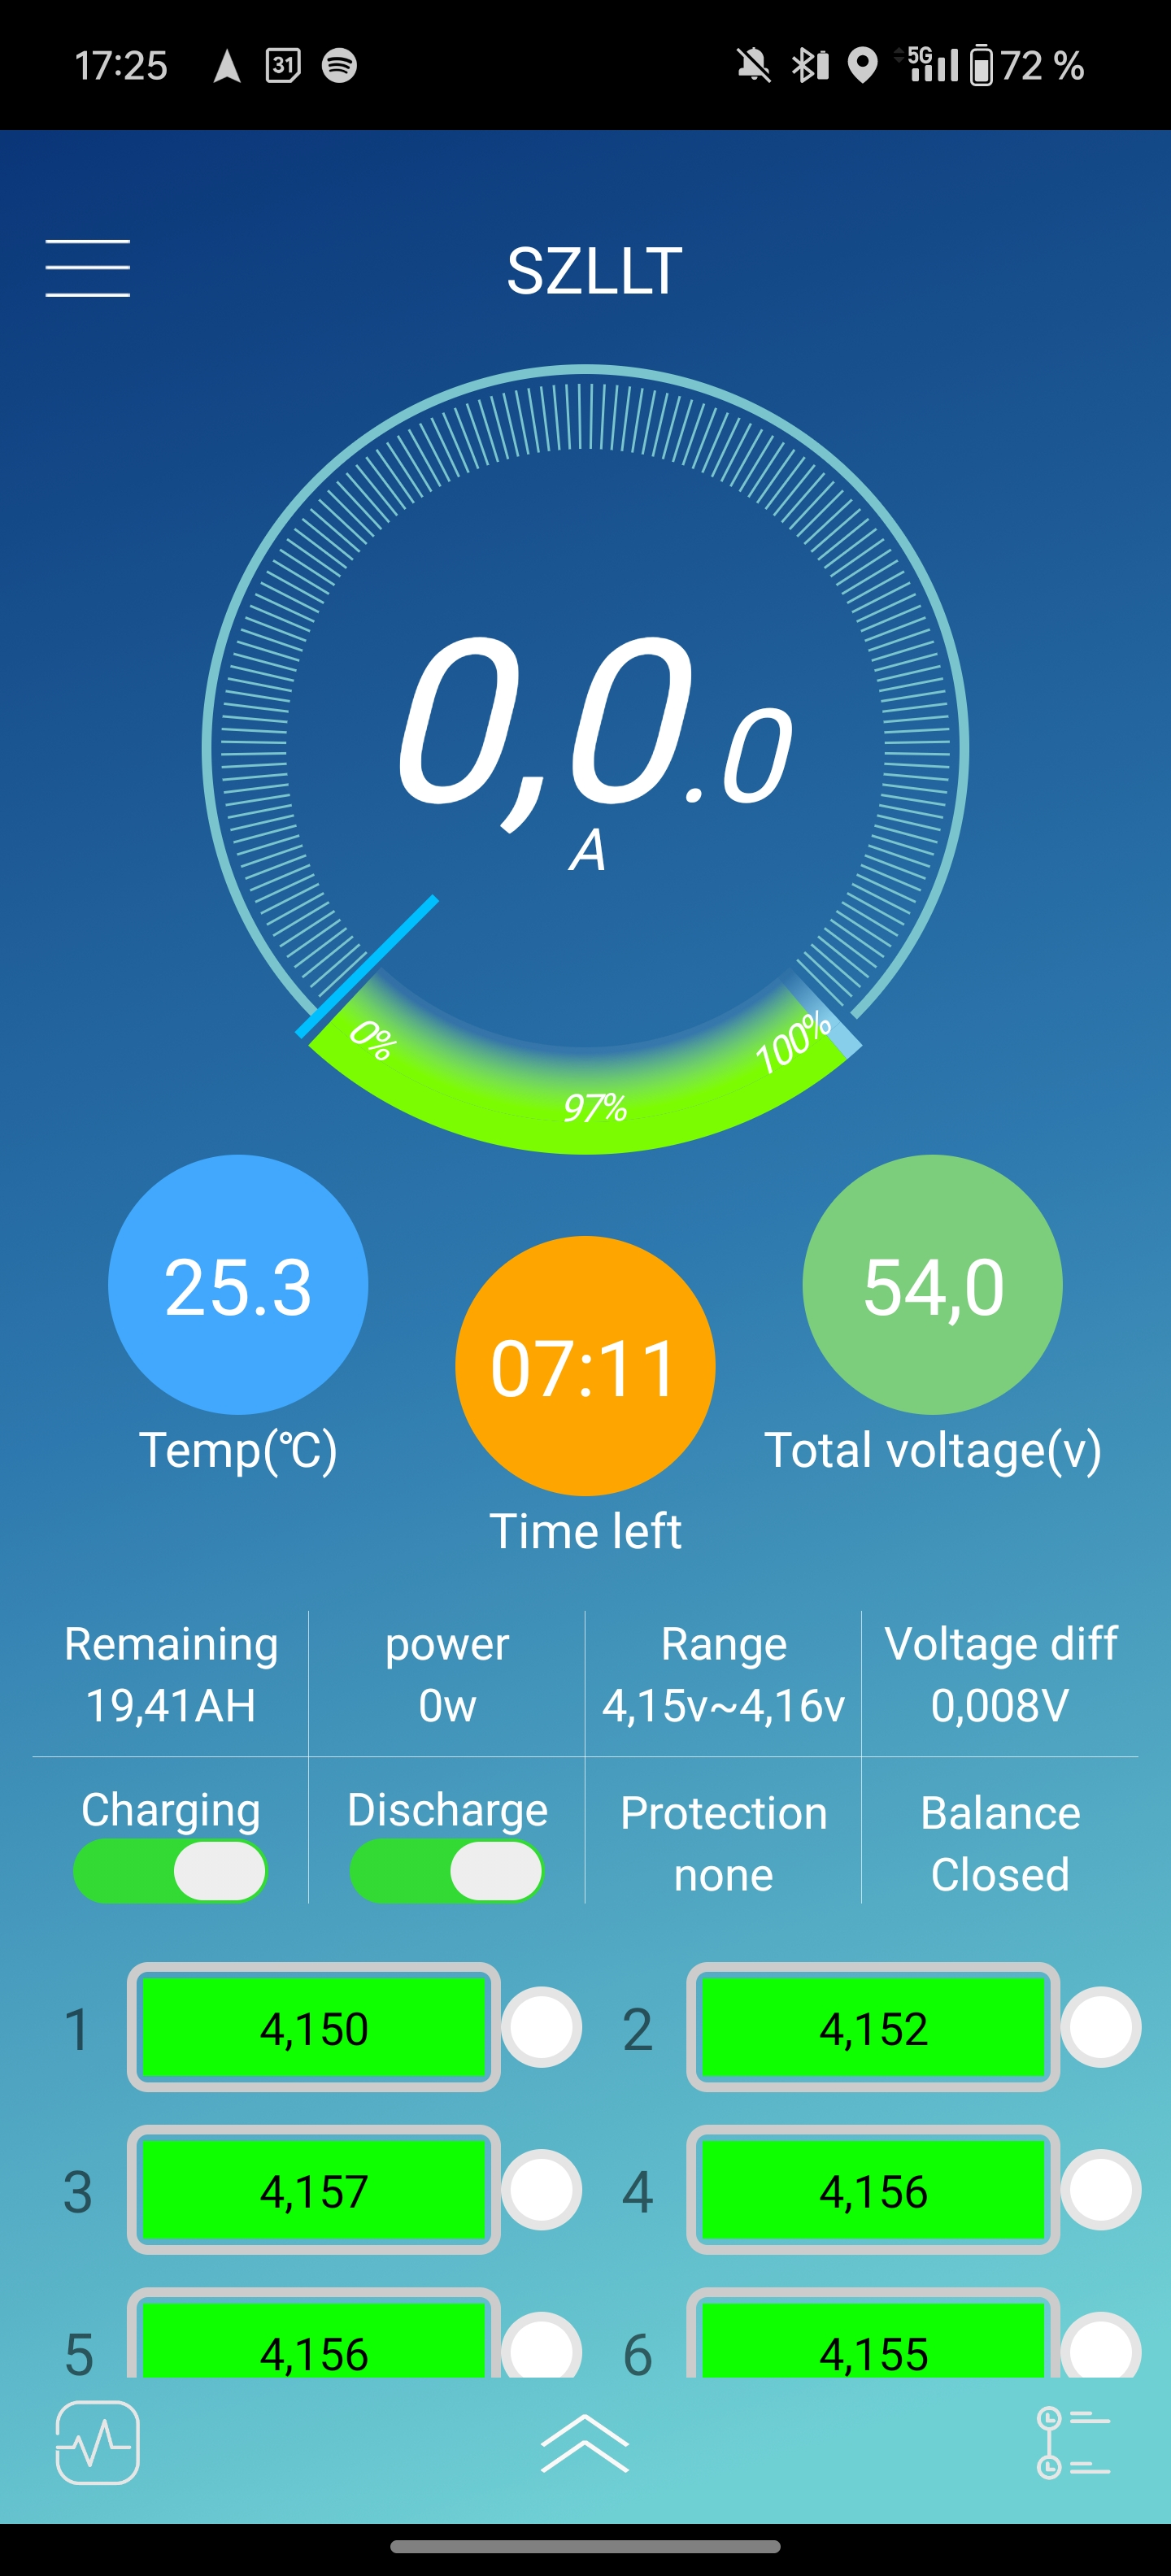
\includegraphics[width=10cm]{images/BMSvorderFahrt}
    \caption{Batterie-Stand vor der Fahrt\cite{lorenz_scherrer_selbst_2023}}
    \label{fig:31}
\end{figure}

\begin{figure}[h]
    \centering
    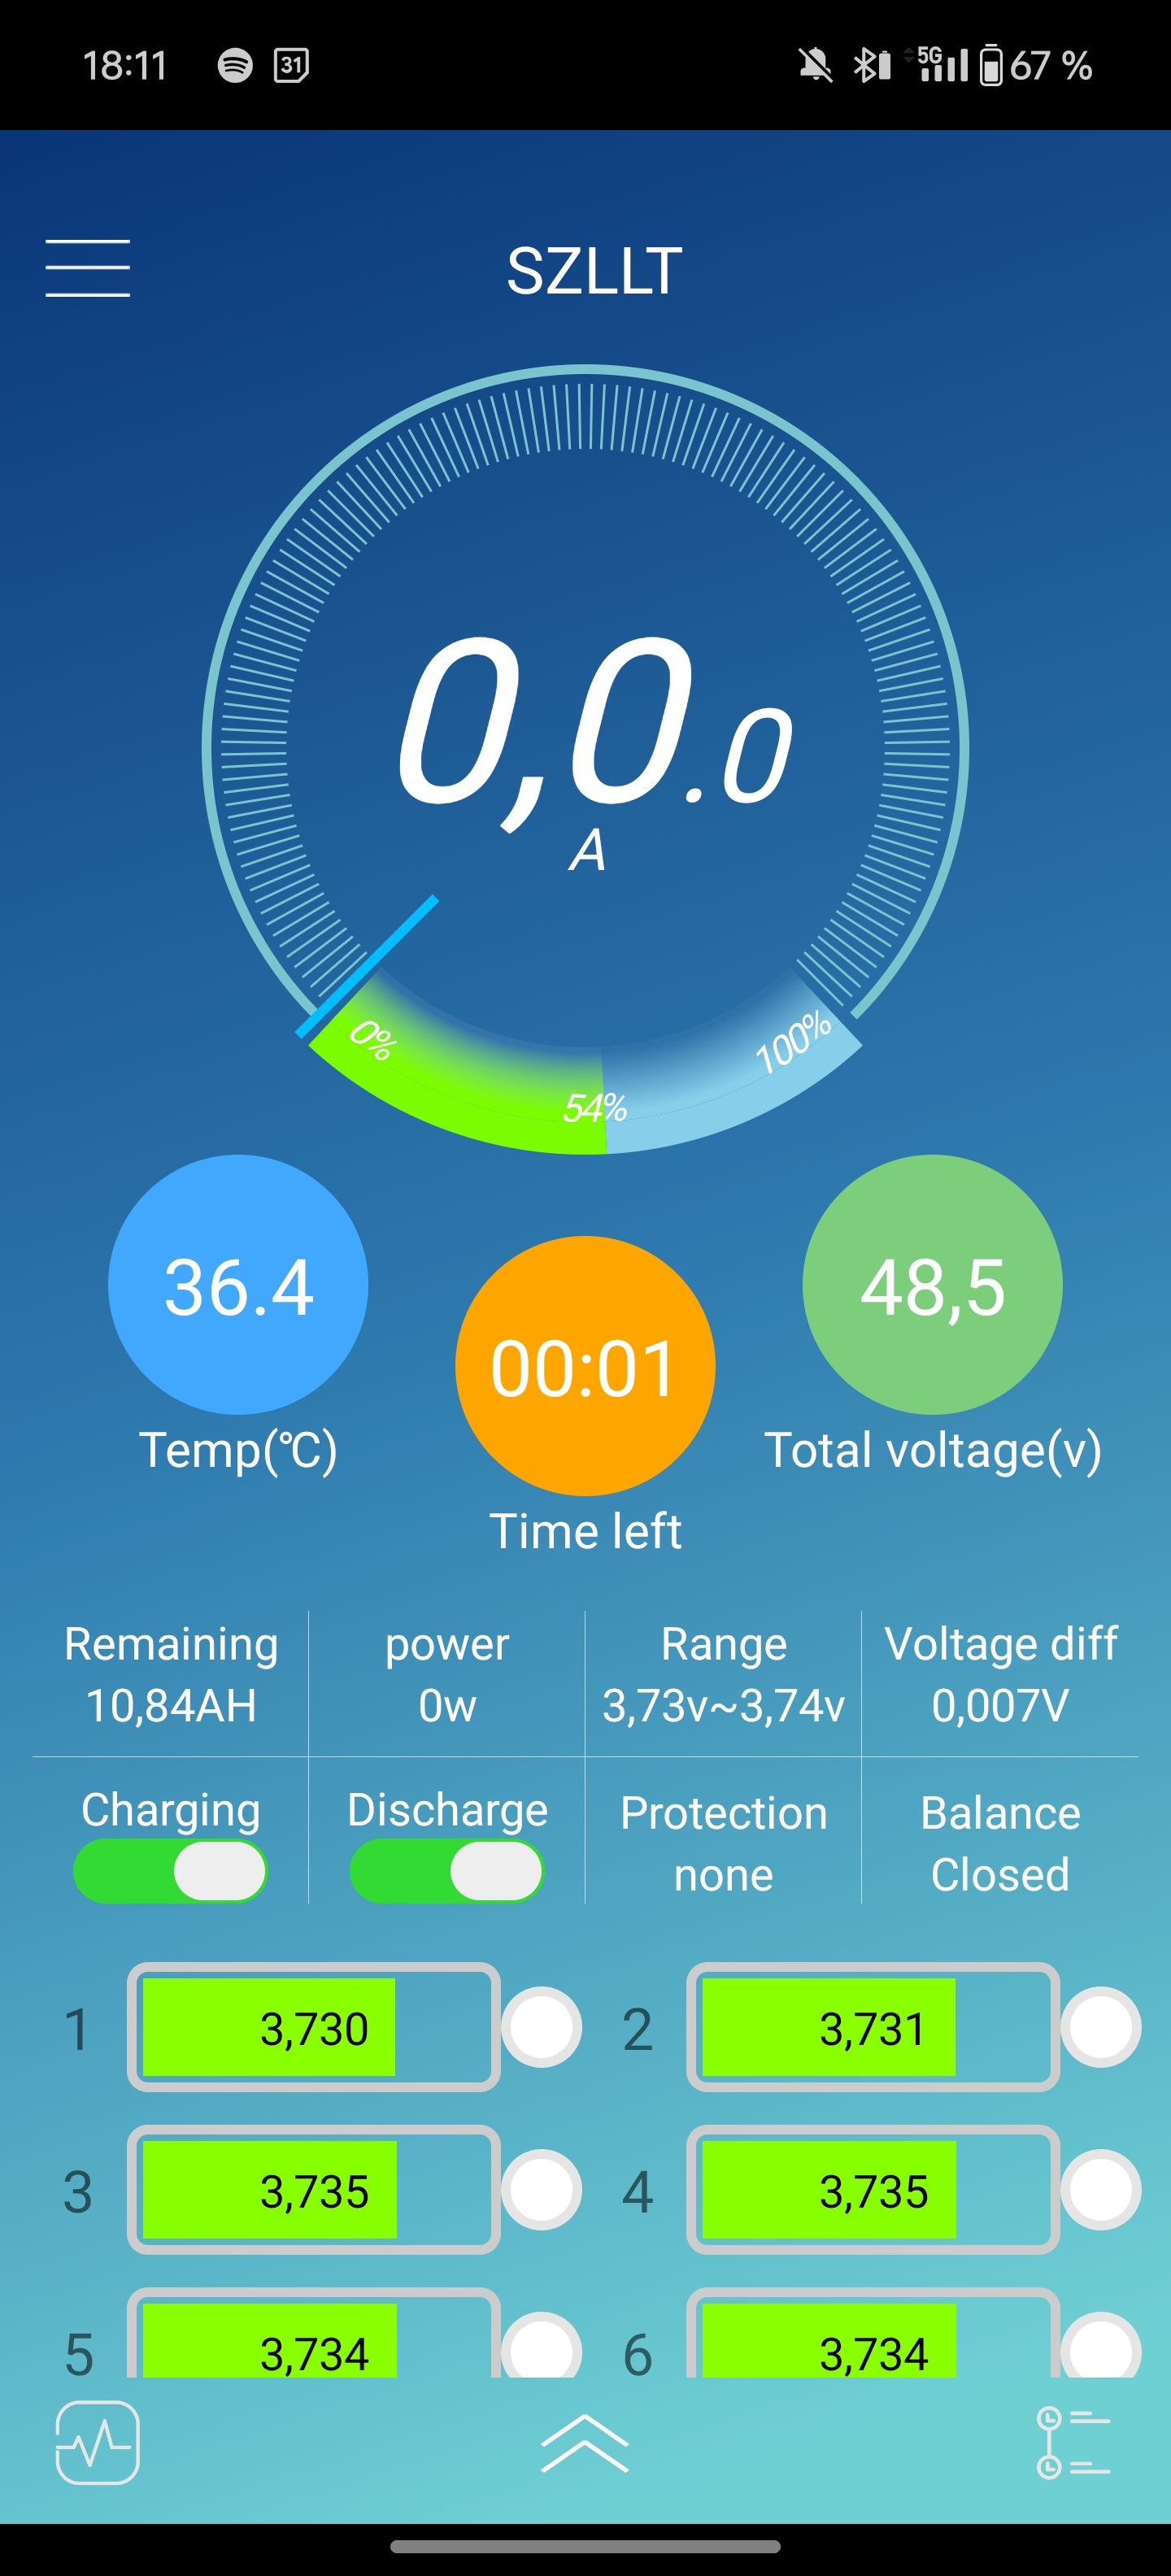
\includegraphics[width=10cm]{images/BMSnachderFahrt}
    \caption{Batterie Stand nach der Fahrt\cite{lorenz_scherrer_selbst_2023}}
    \label{fig:32}
\end{figure}

\begin{figure}[h]
    \centering
    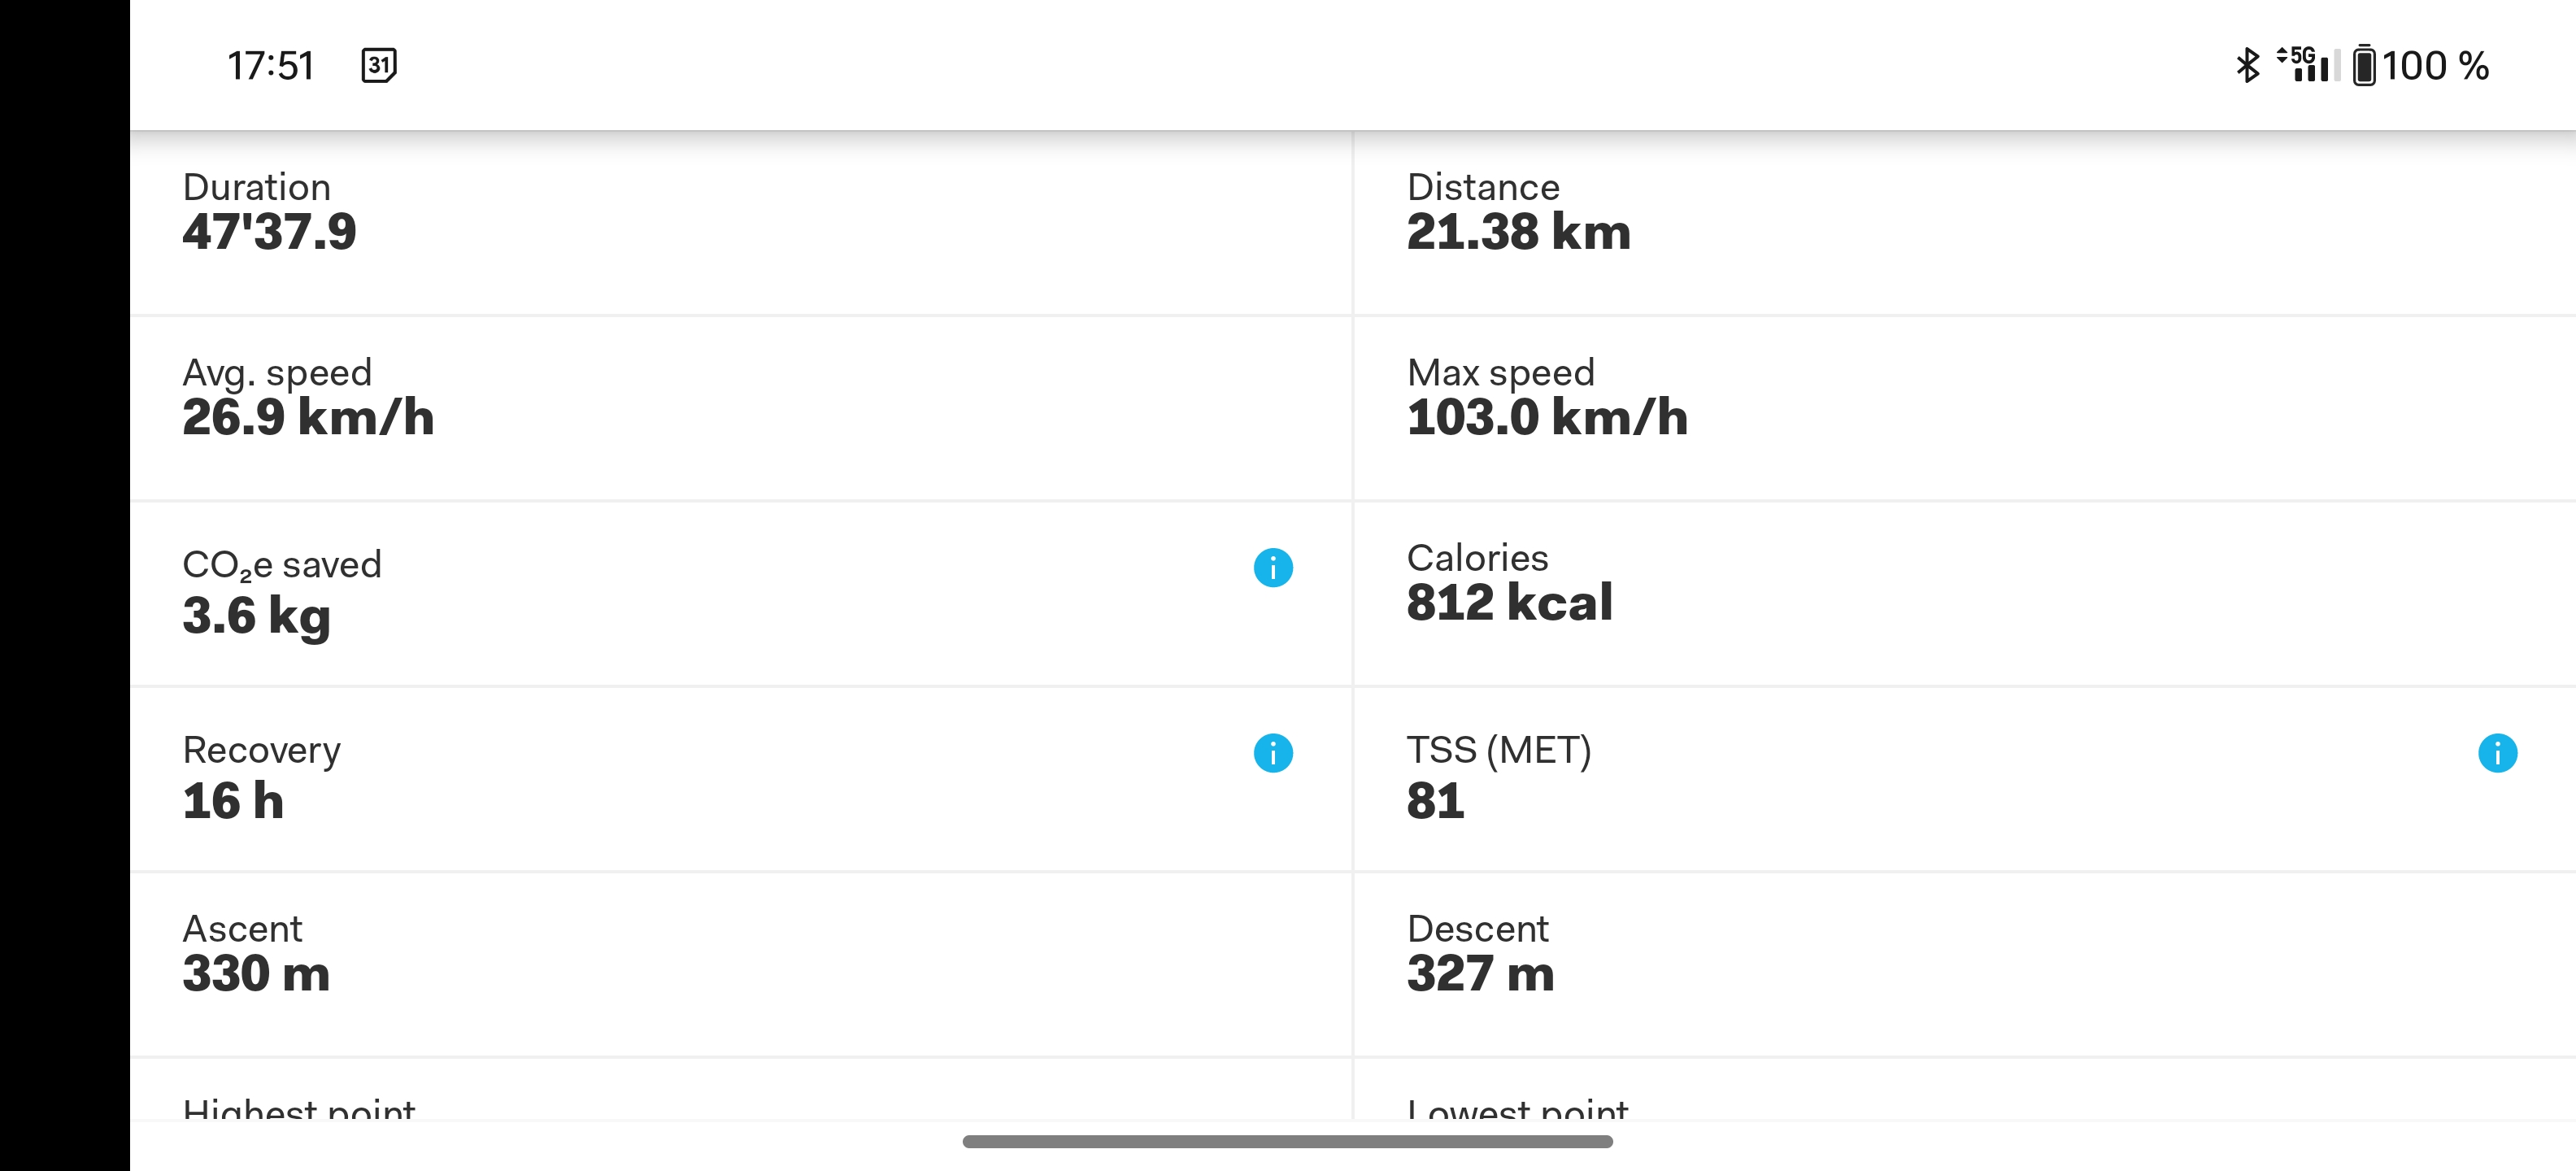
\includegraphics[width=10cm]{images/streckenparameter}
    \caption{Streckenparameter\cite{lorenz_scherrer_selbst_2023}}
    \label{fig:33}
\end{figure}

\begin{figure}[h]
    \centering
    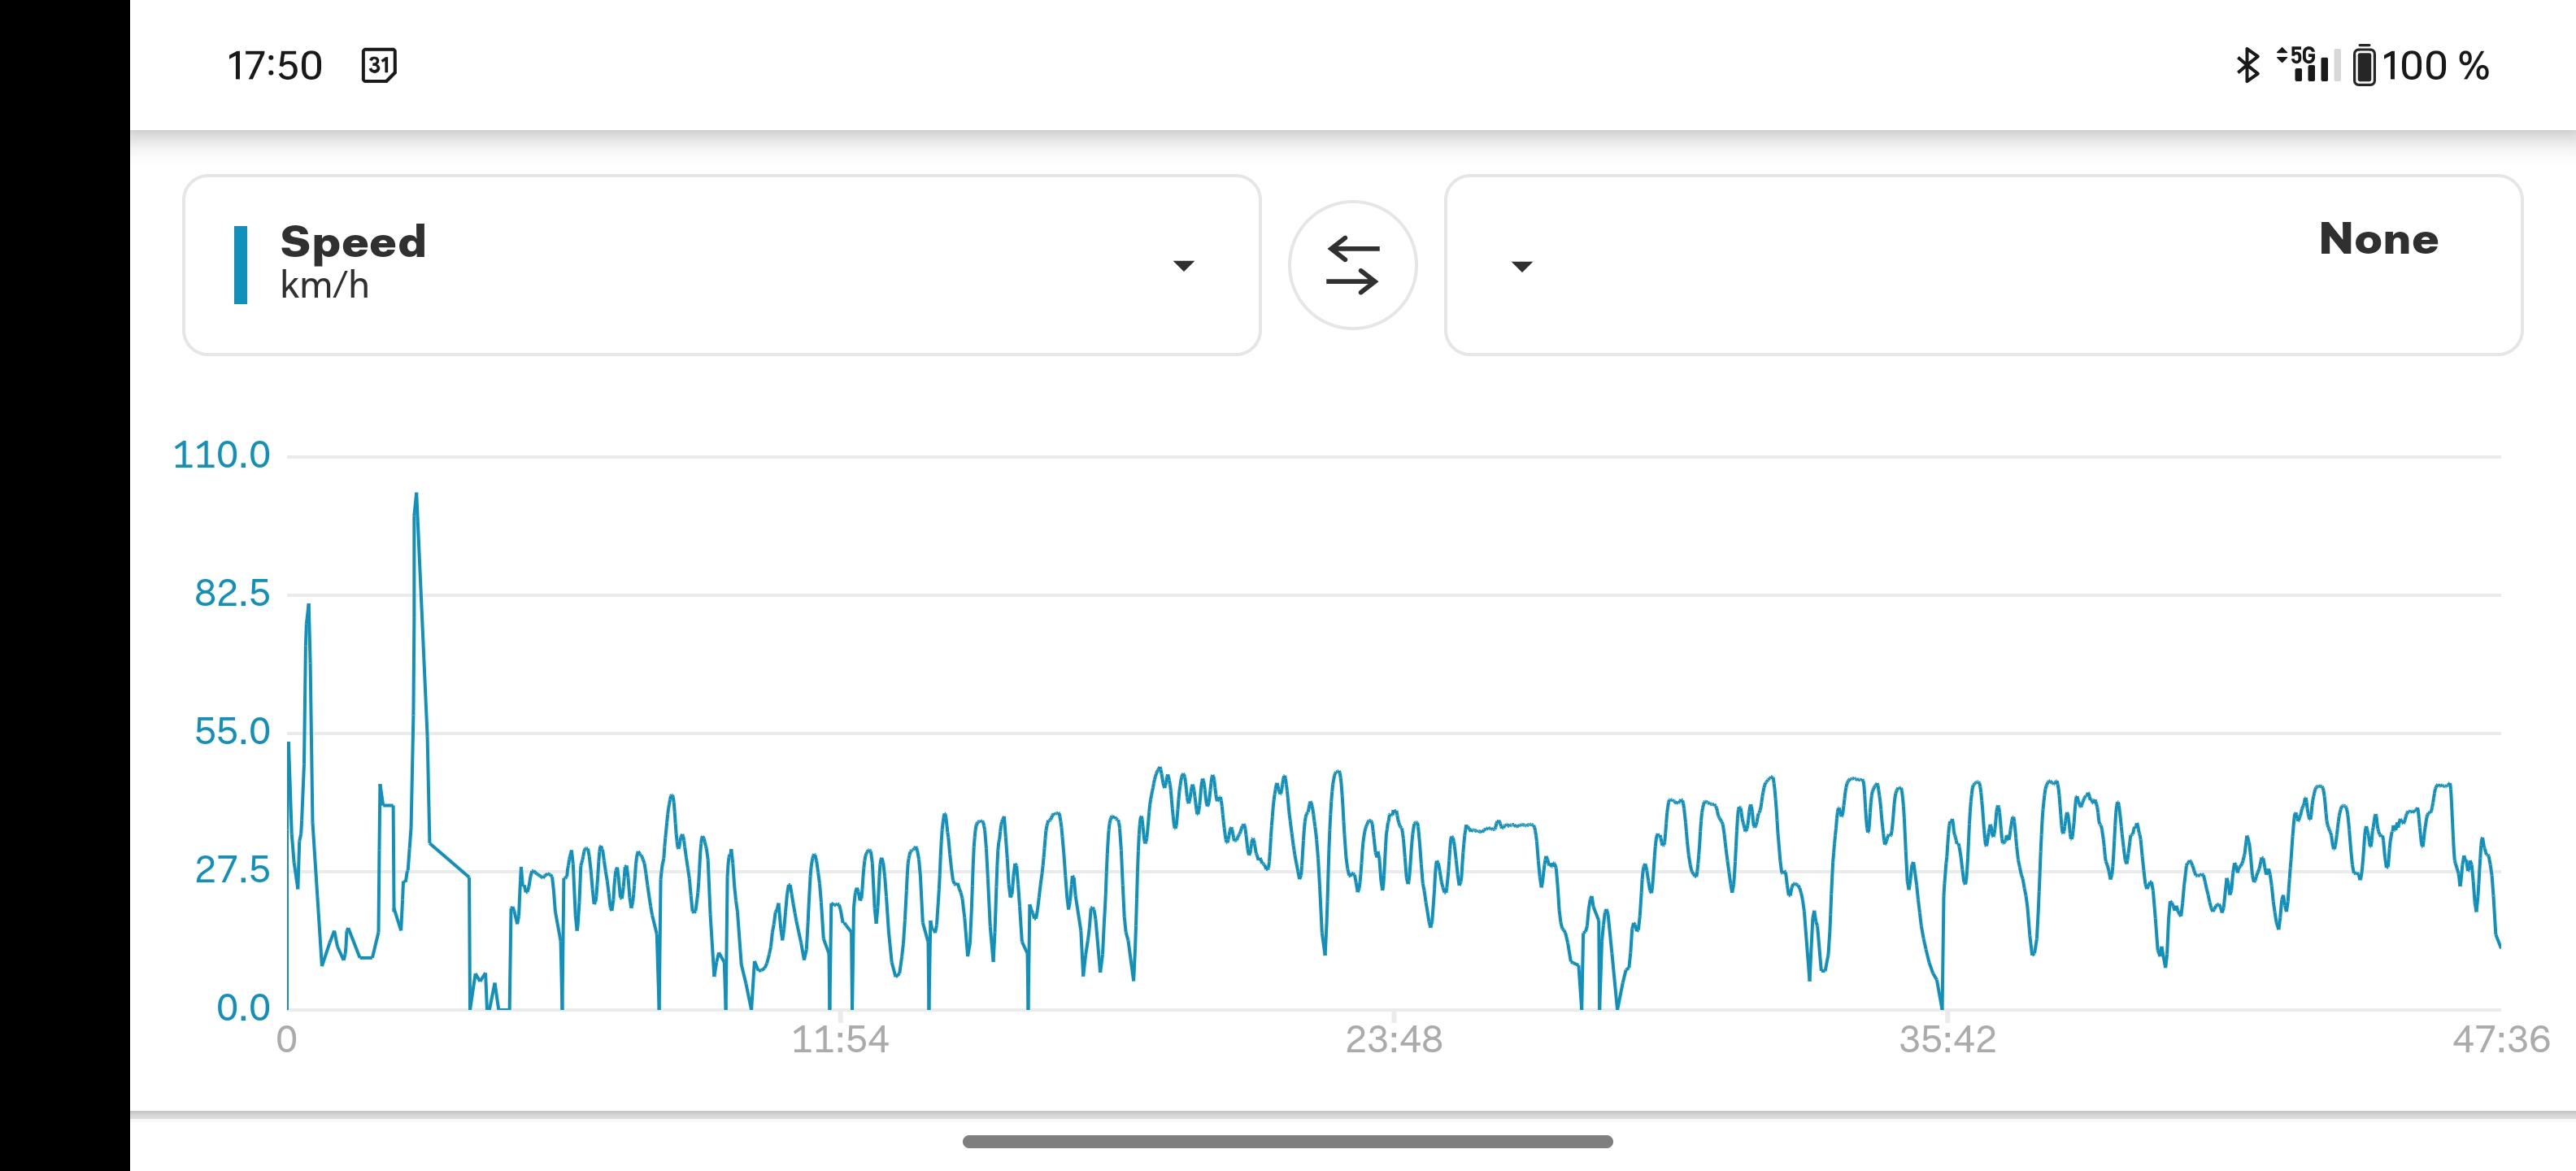
\includegraphics[width=10cm]{images/Geschwindigkeitshistogramm}
    \caption{Geschwindigkeitshistogramm\cite{lorenz_scherrer_selbst_2023}}
    \label{fig:34}
\end{figure}

\begin{figure}[h]
    \centering
    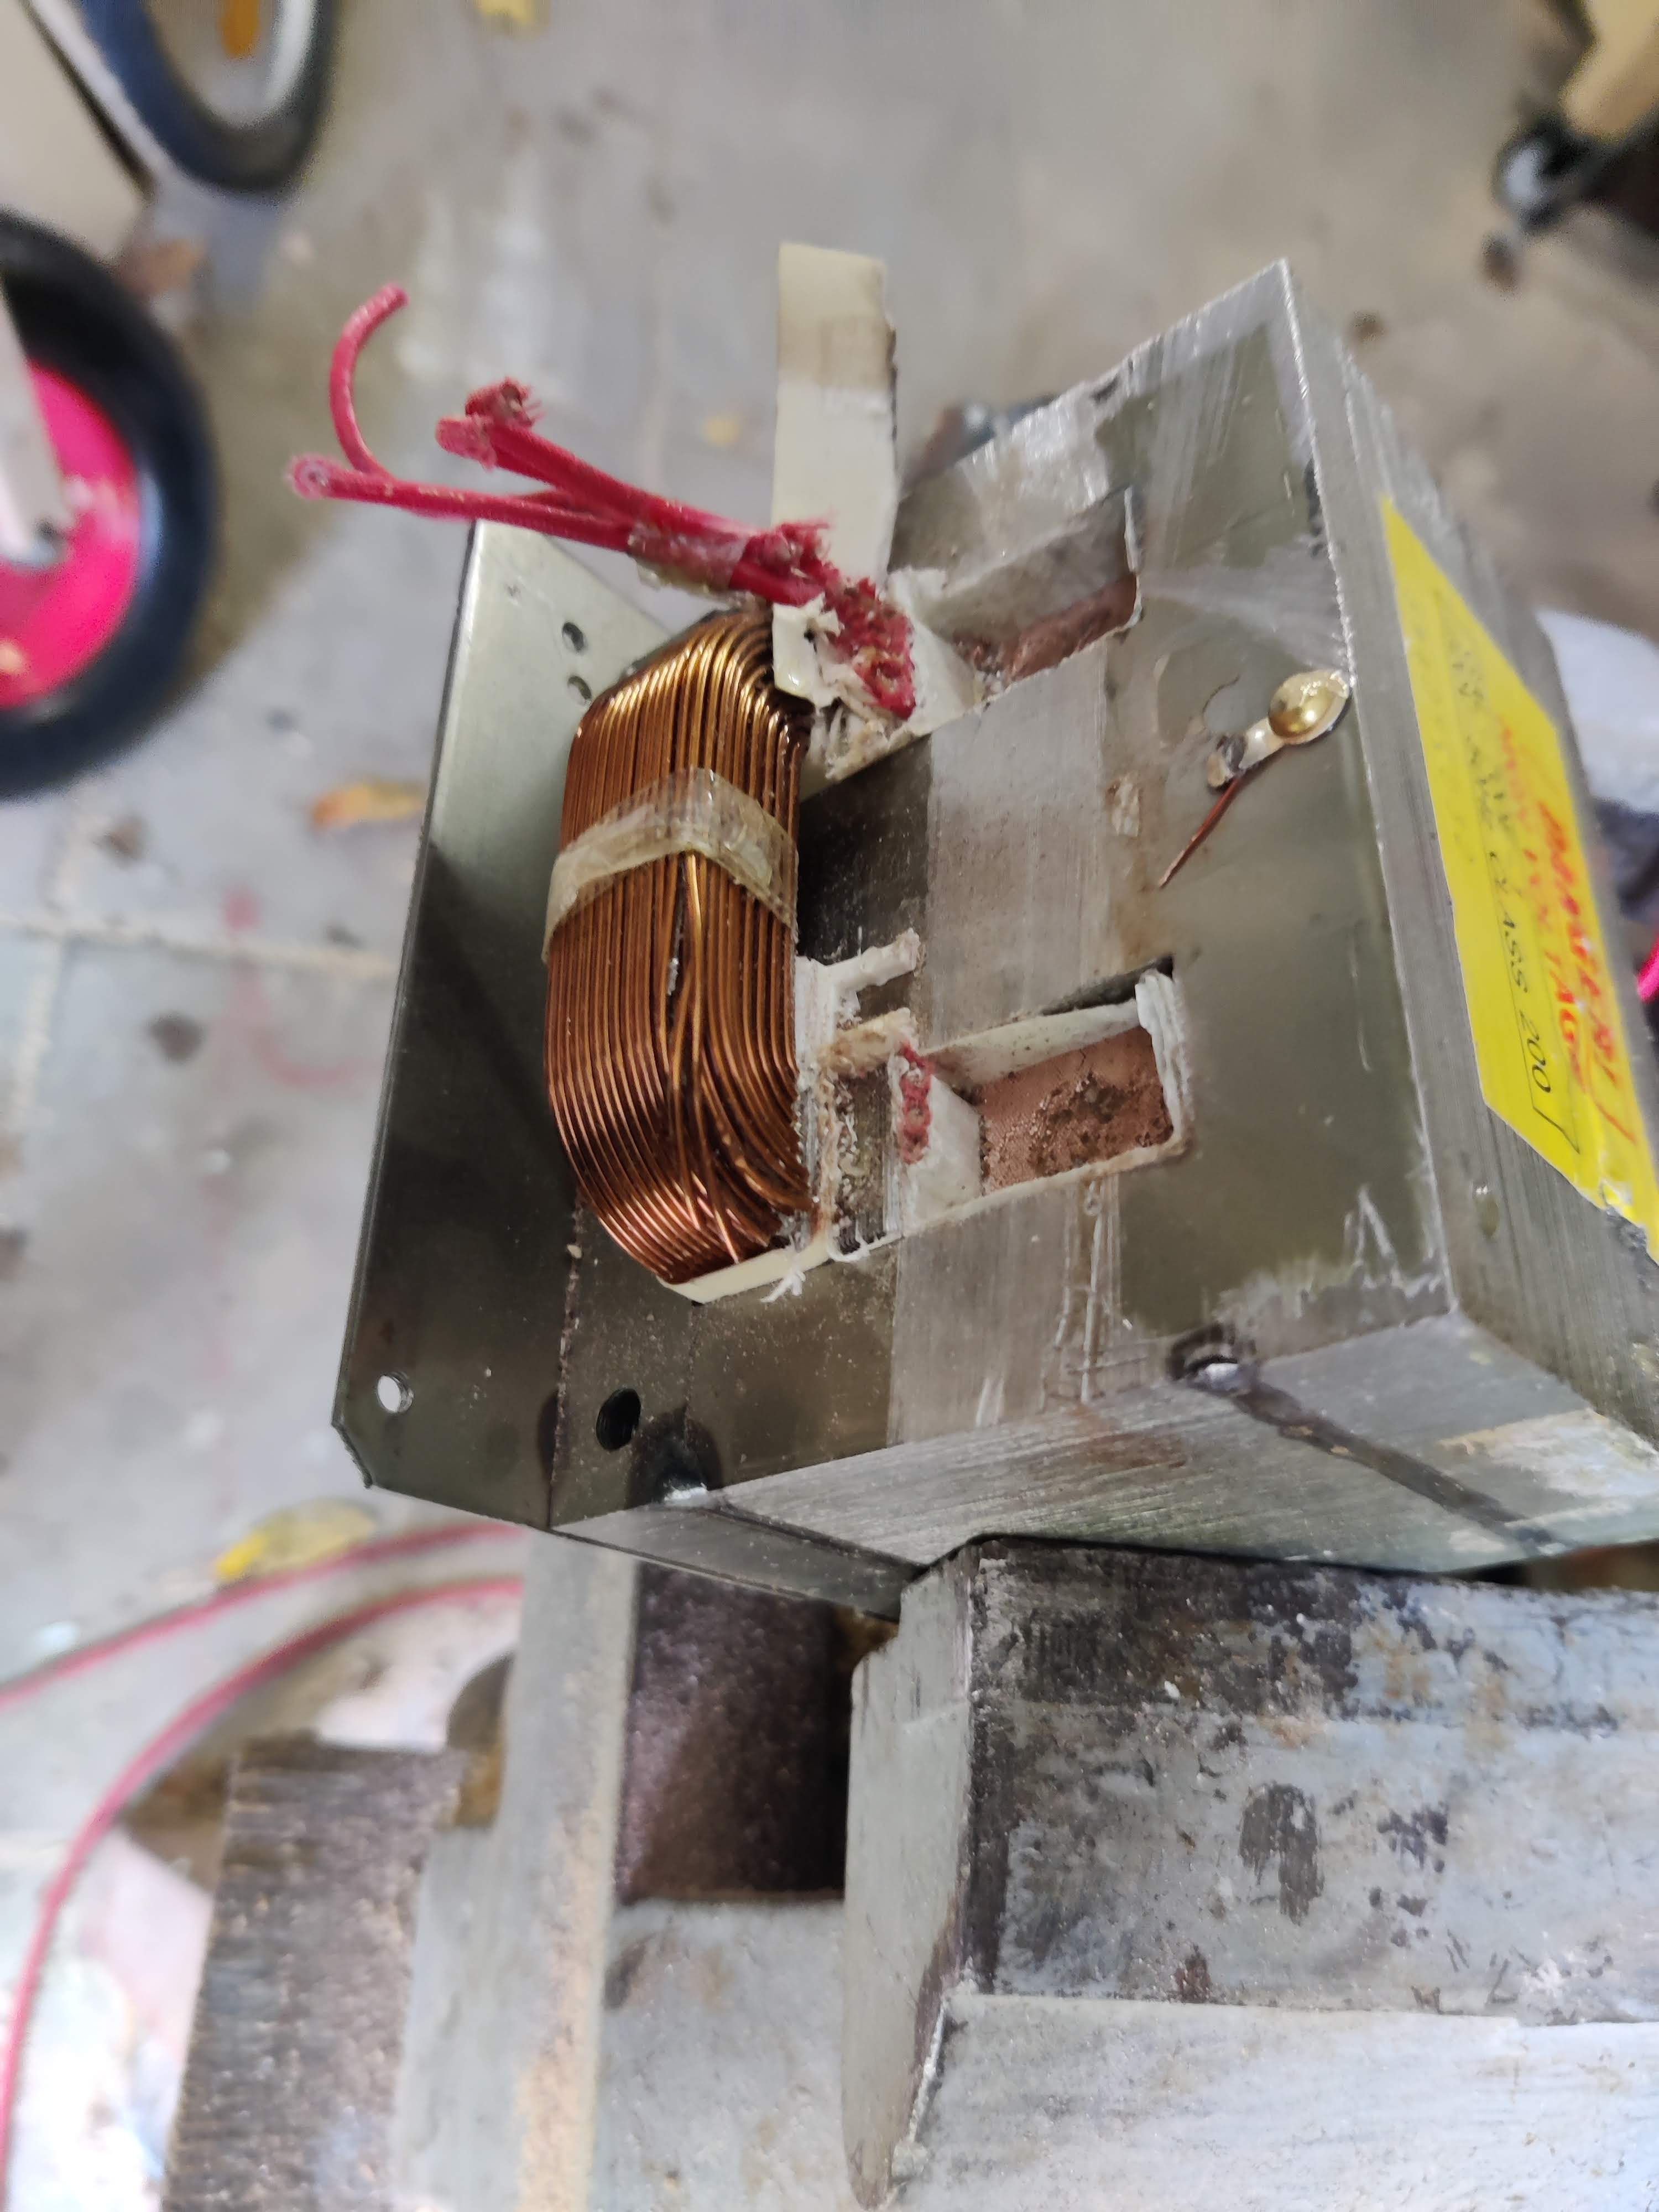
\includegraphics[width=10cm]{images/KaputterTransformator}
    \caption{Kaputter primärer Block\cite{lorenz_scherrer_selbst_2023}}
    \label{fig:35}
\end{figure}

\subsection*{Allgemeine Grundeinstellungen}\label{sec:parameter}
\begin{enumerate}[label=\arabic*.]
    \item Maximale Fahrgeschwindigkeit
    \item Rad-Durchmesser
    \item Metrische und imperiale Einheiten
\end{enumerate}

\section{P-Parameter-Einstellung}
\begin{enumerate}[label=\arabic*.]
    \item P1 Motorumdrehung Einstellung (Alnico-Zahl)
    \item P2 Geschwindigkeitssignal Einstellung
    \item P3 Motor Unterstützungsmodus
    \item P4 Daumengas Startmodus
    \item P5 Batterie - Ladezustandsanzeige
\end{enumerate}

\section{C-Parameter-Einstellung}
\begin{enumerate}[label=\arabic*.]
    \item C1 PAS - Sensor Parametereinstellung
    \item C2 Motor Phasen Anpassung
    \item C3 Einstellung der Anzahl der Unterstützungsstufen
    \item C4 Daumengas Funktionseinstellung
    \item C5-Controller maximale Stromeinstellung
    \item C6-Hintergrundbeleuchtung Helligkeitseinstellung
    \item C7 Cruise Funktionseinstellung
    \item C8 Motor Betriebstemperatur Anzeige
    \item C9 Power on Passwort Einstellung
    \item C10 Wiederherstellung Werkseinstellung
    \item C11 Einstellung Übertragungsprotokoll
    \item C12-Controller Unterspannungseinstellung
    \item C13 Bremsenergiegewinnung
    \item C14 Abstimmung der Unterstützungsstufen
\end{enumerate}




\addcontentsline{toc}{chapter}{Index}
\printindex

\addcontentsline{toc}{chapter}{Literaturverzeichnis}

% Haben Sie das "biblatex"-Paket nicht installiert, benutzen Sie folgendes:
% Ohne das "biblatex"-Paket (s. bericht.sty) produziert folgendes
% "deutsche" Zitate in Literaturverzeichnissen gemaß der Norm DIN 1505,
% Teil 2 vom Jan. 1984.
% Die Zitatmarken werden alphabetisch nach Verfassern
% sortiert und sind durch abgekürzte Verfasserbuchstaben plus
% Erscheinungsjahr in eckigen Klammern gekennzeichnet.

% \bibliographystyle{alphadin}
% \bibliography{bericht}

%%%%%%%%%%%%%%%%%%%%%%%%%%%%%%%%%%%%%%%5
% BIBLATEX
% Benutzt man das "biblatex"-Paket, muß man folgendes schreiben:
\def\refname{Literaturverzeichnis}
\printbibliography
%%%%%%%%%%%%%%%%%%%%%%%%%%%%%%%%%%%%%%%5


%%%%%%%%%%%%%%%%%%%%%%%%%%%%%%%%%%%%%%%%%%%%%%%%%%%%%%%%%%%%%%%%%%%%%%%%%%%%%%%%
%% Descr:       Vorlage für Berichte der DHBW-Karlsruhe, Änderungshistorie
%% Author:      Prof. Dr. Jürgen Vollmer, vollmer@dhbw-karlsruhe.de
%% $Id: changelog.tex,v 1.17 2023/07/25 10:47:22 vollmer Exp $
%% -*- coding: utf-8 -*-
%%%%%%%%%%%%%%%%%%%%%%%%%%%%%%%%%%%%%%%%%%%%%%%%%%%%%%%%%%%%%%%%%%%%%%%%%%%%%%%

\chapter*{Änderungen}

\begin{description}
\item[2023/07/25] Seitennummern: Römische Ziffern in Inhaltsverzeichnis etc., dann arabische Ziffern
                  beginnend mit 1: \verb+\pagenumbering{roman}+,
                  \verb+\pagenumbering{arabic}+
\item[2020/03/13] Tippfehler korrigiert\\
                  aktuelle Formulierungen aus der Prüfungsordnung Technik übernommen\\
                  Formatdatei erklärt
\item[2017/10/06] Anpassung an neuer Versionen diverse Pakete.
\item[2016/03/16] Auf UTF-8 umgestellt, Indices.
\item[2010/04/12] ToDo-Markierungen mit dem \verb+\todo+-Kommando.
\item[2010/01/27] Anhang (\texttt{appendix}), Selbständigkeits-Erklärung, \texttt{framed}-Paket.
\item[2010/01/21] Abkürzungen (\texttt{acronym}), \texttt{table} und \texttt{tabular} benutzt,
     unübliche Pakete beigelegt.
\item[2010/01/18] Code-Listings (\texttt{listings}), Literaturreferenzen \texttt{biblatex})
\item[2010/01/11] Initiale Version.
\end{description}


\newpage
\addcontentsline{toc}{chapter}{Liste der ToDo's}
%\listoftodos[Liste der ToDo's]


\end{document}
